% !TeX encoding = UTF-8
\documentclass[aspectratio=169]{beamer}
\useoutertheme[progressbar=frametitle]{metropolis}
\useinnertheme{metropolis}
\definecolor{nabgray}{rgb}{0.6,0.59,0.61}
\usecolortheme[named=nabgray]{structure}

\usepackage{tikz}
\usepackage[utf8]{inputenc}
\usepackage[spanish]{babel}
\usepackage{fontspec}
\setmonofont{JetBrains Mono}
\setmainfont{Roboto}
\setsansfont{Roboto}

\usepackage{smartdiagram}
\usepackage{qtree}
\usepackage{verbatim}
\usepackage{svg}
\usepackage{graphicx}
\usepackage{color}

\definecolor{lightgray}{rgb}{0.95, 0.95, 0.95}
\definecolor{darkgray}{rgb}{0.4, 0.4, 0.4}
%\definecolor{purple}{rgb}{0.65, 0.12, 0.82}
\definecolor{editorGray}{rgb}{0.95, 0.95, 0.95}
\definecolor{editorOcher}{rgb}{1, 0.5, 0} % #FF7F00 -> rgb(239, 169, 0)
\definecolor{editorGreen}{rgb}{0, 0.5, 0} % #007C00 -> rgb(0, 124, 0)
\definecolor{orange}{rgb}{1,0.45,0.13}
\definecolor{olive}{rgb}{0.17,0.59,0.20}
\definecolor{brown}{rgb}{0.69,0.31,0.31}
\definecolor{purple}{rgb}{0.38,0.18,0.81}
\definecolor{lightblue}{rgb}{0.1,0.57,0.7}
\definecolor{lightred}{rgb}{1,0.4,0.5}
\usepackage{upquote}
\usepackage{listings}
\lstset{language=java,
	basicstyle=\footnotesize\ttfamily,
	keywordstyle=\footnotesize\color{blue}\ttfamily,
	escapeinside={<@}{@>}
}


\usebackgroundtemplate%
{%
	
\includegraphics[width=\paperwidth]{Images/Contenido}%
}


\title{Patrones de Cloud Native con MicroProfile}
\author{Víctor Orozco}
\institute{Nabenik}
\date{\today}

\begin{document}
{
    \usebackgroundtemplate{
\includegraphics[width=\paperwidth]{Images/portada}}
    \setbeamercolor{frametitle}{fg=red}
    \usebeamercolor[fg]{normal text}
    \frame{\titlepage}
}


{
    \usebackgroundtemplate{
\includegraphics[width=\paperwidth]{Images/separador}}
    \setbeamercolor{normal text}{fg=white}
    \setbeamercolor{frametitle}{fg=red}
    \usebeamercolor[fg]{normal text}
    \section{Patrones de microservicios}
}


\begin{frame}{Microservicios = Metapatron arquitectural}
	
	Arquitectura que estructura una aplicación como un conjunto de servicios débilmente acoplados. Corresponde al eje Y del scale cube cuyo objetivo final son sistemas reactivos
	
	\begin{figure}
		\centering
		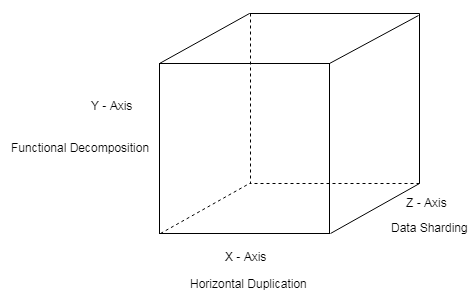
\includegraphics[width=0.6\linewidth]{Images/scale}
	\end{figure}
	
\end{frame}

\begin{frame}{}
	
	\begin{figure}
		\centering
		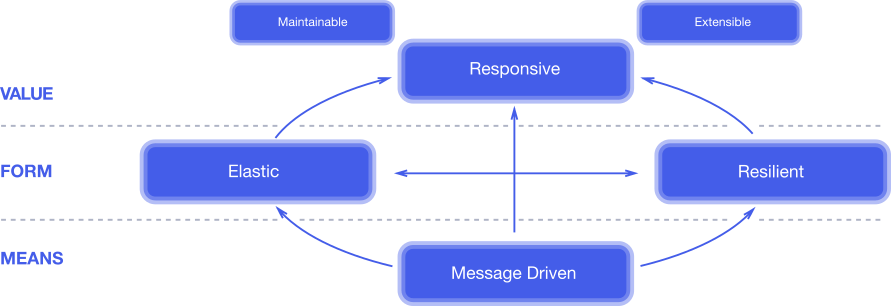
\includegraphics[width=\linewidth]{Images/reactive-traits.png}
	\end{figure}
	
\end{frame}


\begin{frame}{Application Server}
	
	\begin{itemize}
		\item Transacionalidad distribuida (JTA/XA)
		\item Contratos (JNDI)
		\item Service discovery (JNDI)
		\item Deployment (EAR/Class Loaders/Dashboards)
		\item Métricas (JMX)
		\item Seguridad (SoteriaRI/JACC)
	\end{itemize}
	
\end{frame}



\begin{frame}{Microservicios}
	
	Aplicaciones Cloud Native
	\begin{itemize}
		\item Sistemas reactivos
		\item 12 factores Cloud Native
		\item Design patterns
		\item Domain Driven Design
		\item Microservice chassis y service mesh
		\item Orquestación de contenedores
	\end{itemize}
	
\end{frame}


\begin{frame}{Microservicios = Metapatron arquitectural}
	
	Cloud Native
	\begin{itemize}
		\item (Nos gustan) Sistemas reactivos
		\item (Es posible mediante los) 12 factores Cloud Native
		\item (Usamos soluciones probada con) design patterns
		\item (Fragmentamos le sistema mediante) Domain Driven Design
		\item \textbf{(Implementamos los servicios com frameworks) microservice chassis y service mesh}
		\item (Hacemos despliegue) mediante orquestación de contenedores
	\end{itemize}
	
\end{frame}

\begin{frame}{}
\begin{figure}
	\centering
	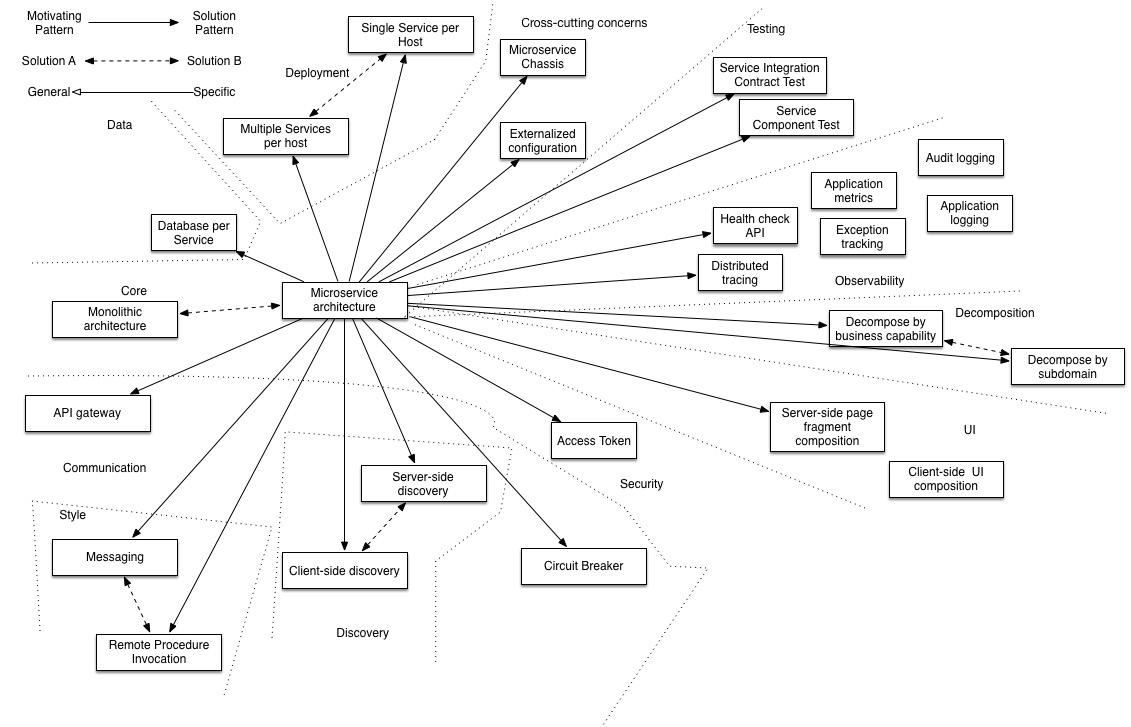
\includegraphics[width=\linewidth]{Images/PatternsRelatedToMicroservices}
\end{figure}
\end{frame}

\begin{frame}{}
\begin{figure}
	\centering
	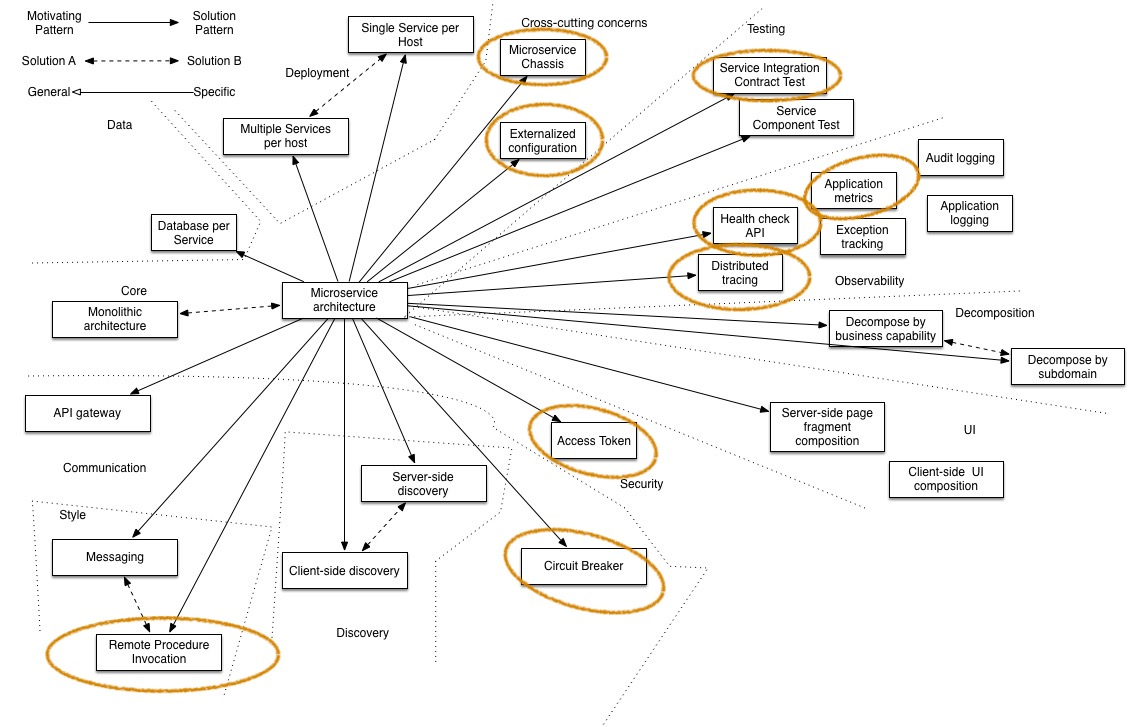
\includegraphics[width=\linewidth]{Images/PatternsRelatedToMicroservices2}
\end{figure}
\end{frame}



{
    \usebackgroundtemplate{
\includegraphics[width=\paperwidth]{Images/separador}}
    \setbeamercolor{normal text}{fg=white}
    \setbeamercolor{frametitle}{fg=red}
    \usebeamercolor[fg]{normal text}
    \section{Eclipse MicroProfile}
}


\begin{frame}{Eclipse MicroProfile}
\begin{figure}
	\centering
	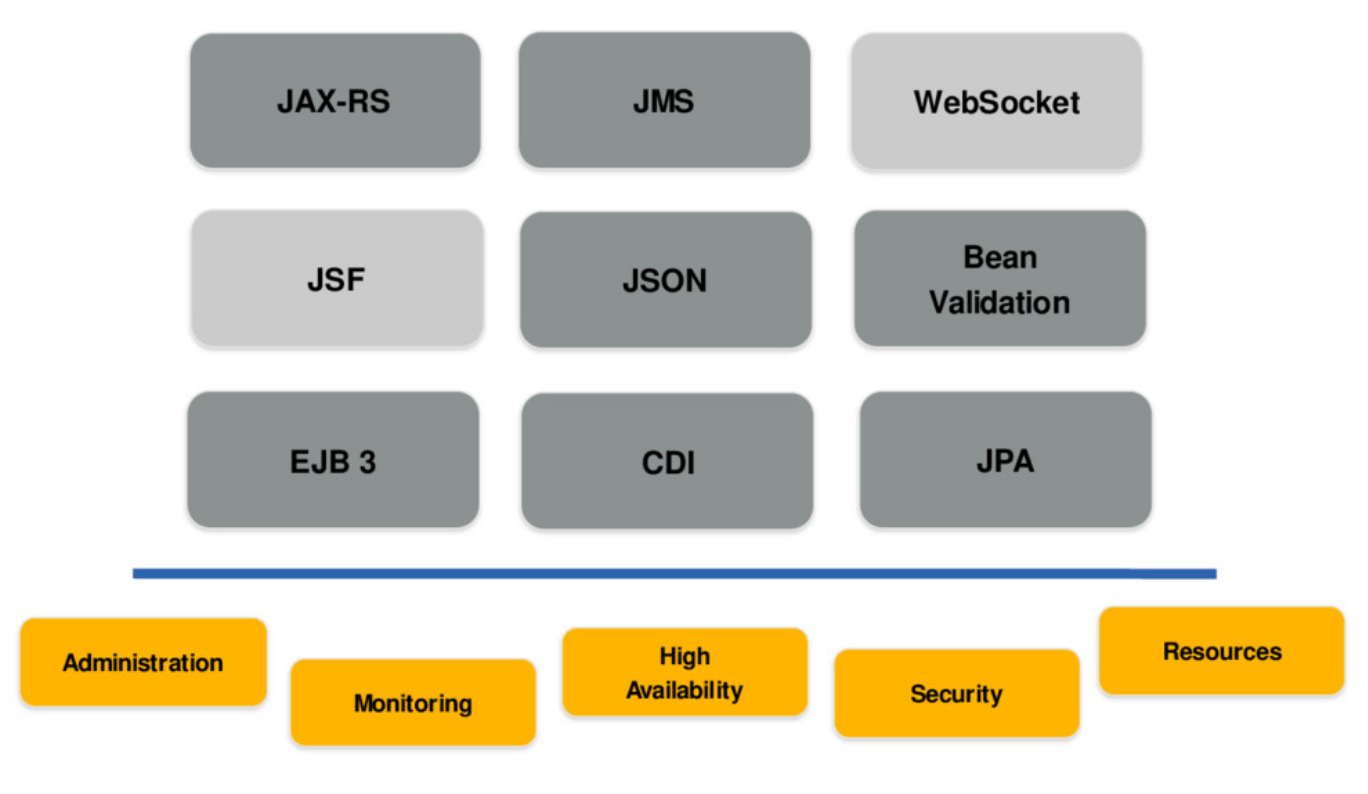
\includegraphics[width=0.8\linewidth]{Images/javaeemicropancake}
	\caption{Credito: Reza Rahman}
\end{figure}
\end{frame}

\begin{frame}{Eclipse MicroProfile}
	\begin{figure}
		\centering
		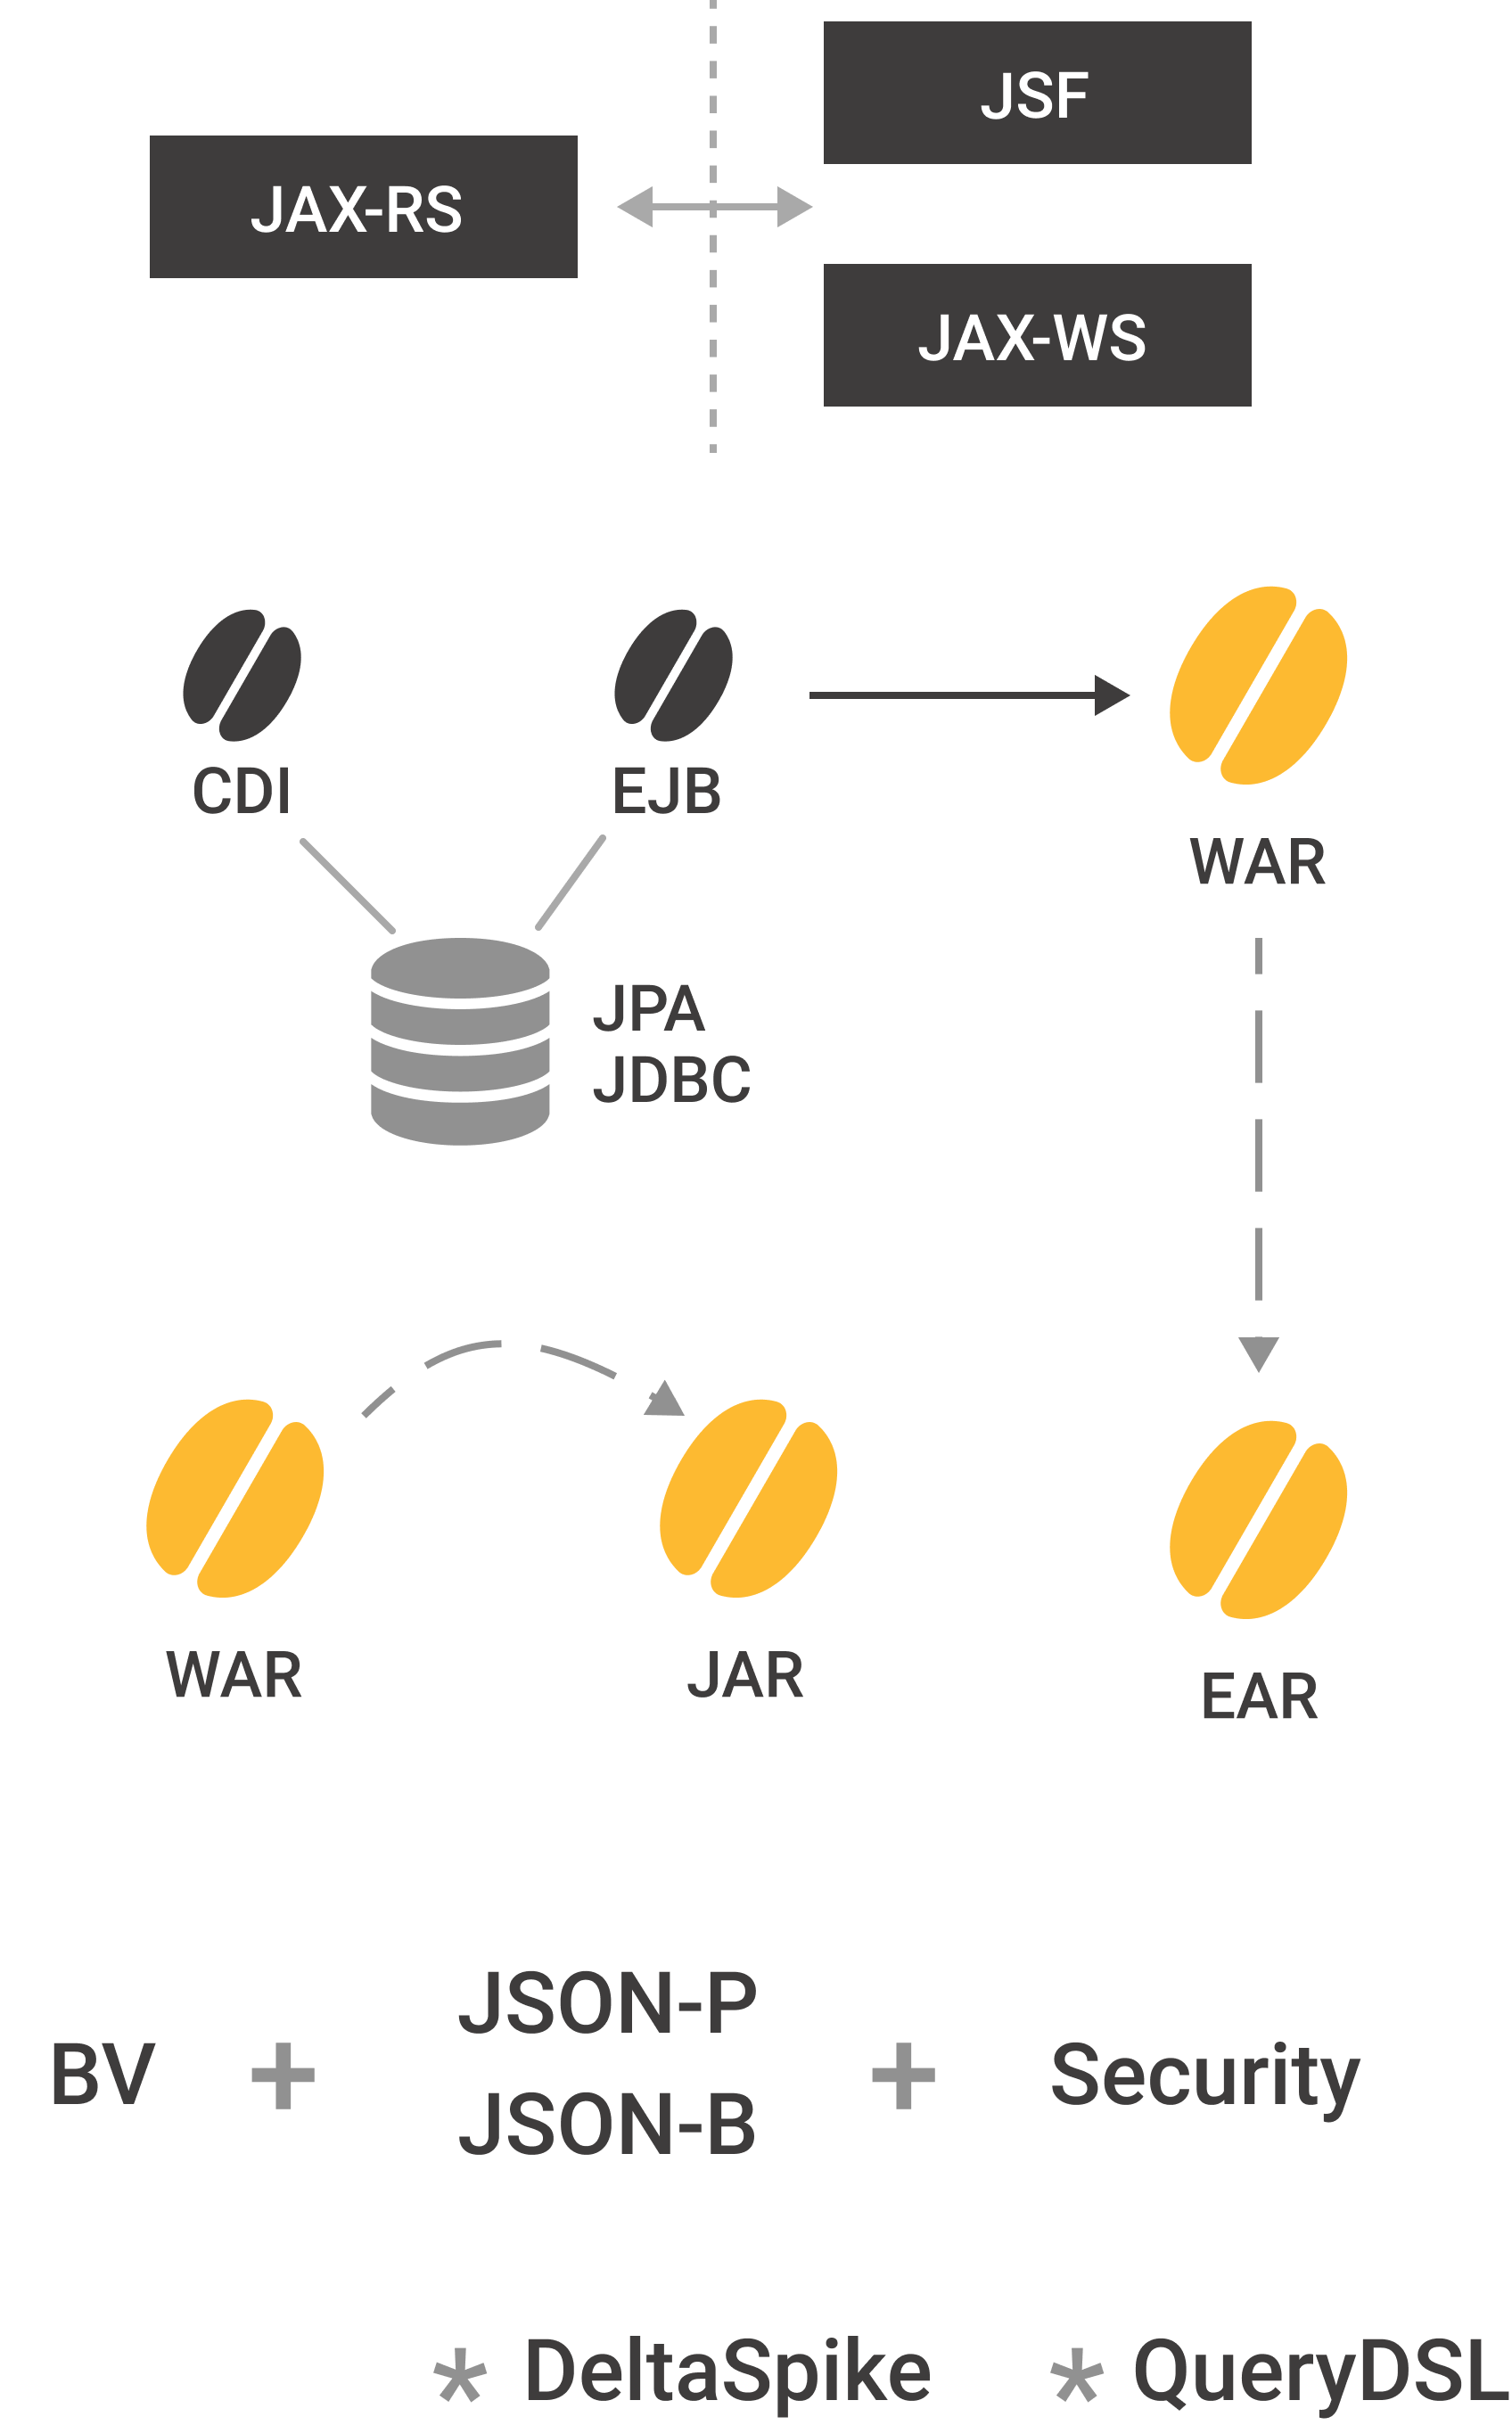
\includegraphics[width=0.4\linewidth]{Images/oldsetup}
	\end{figure}
\end{frame}

\begin{frame}{Eclipse MicroProfile}
\begin{figure}
	\centering
	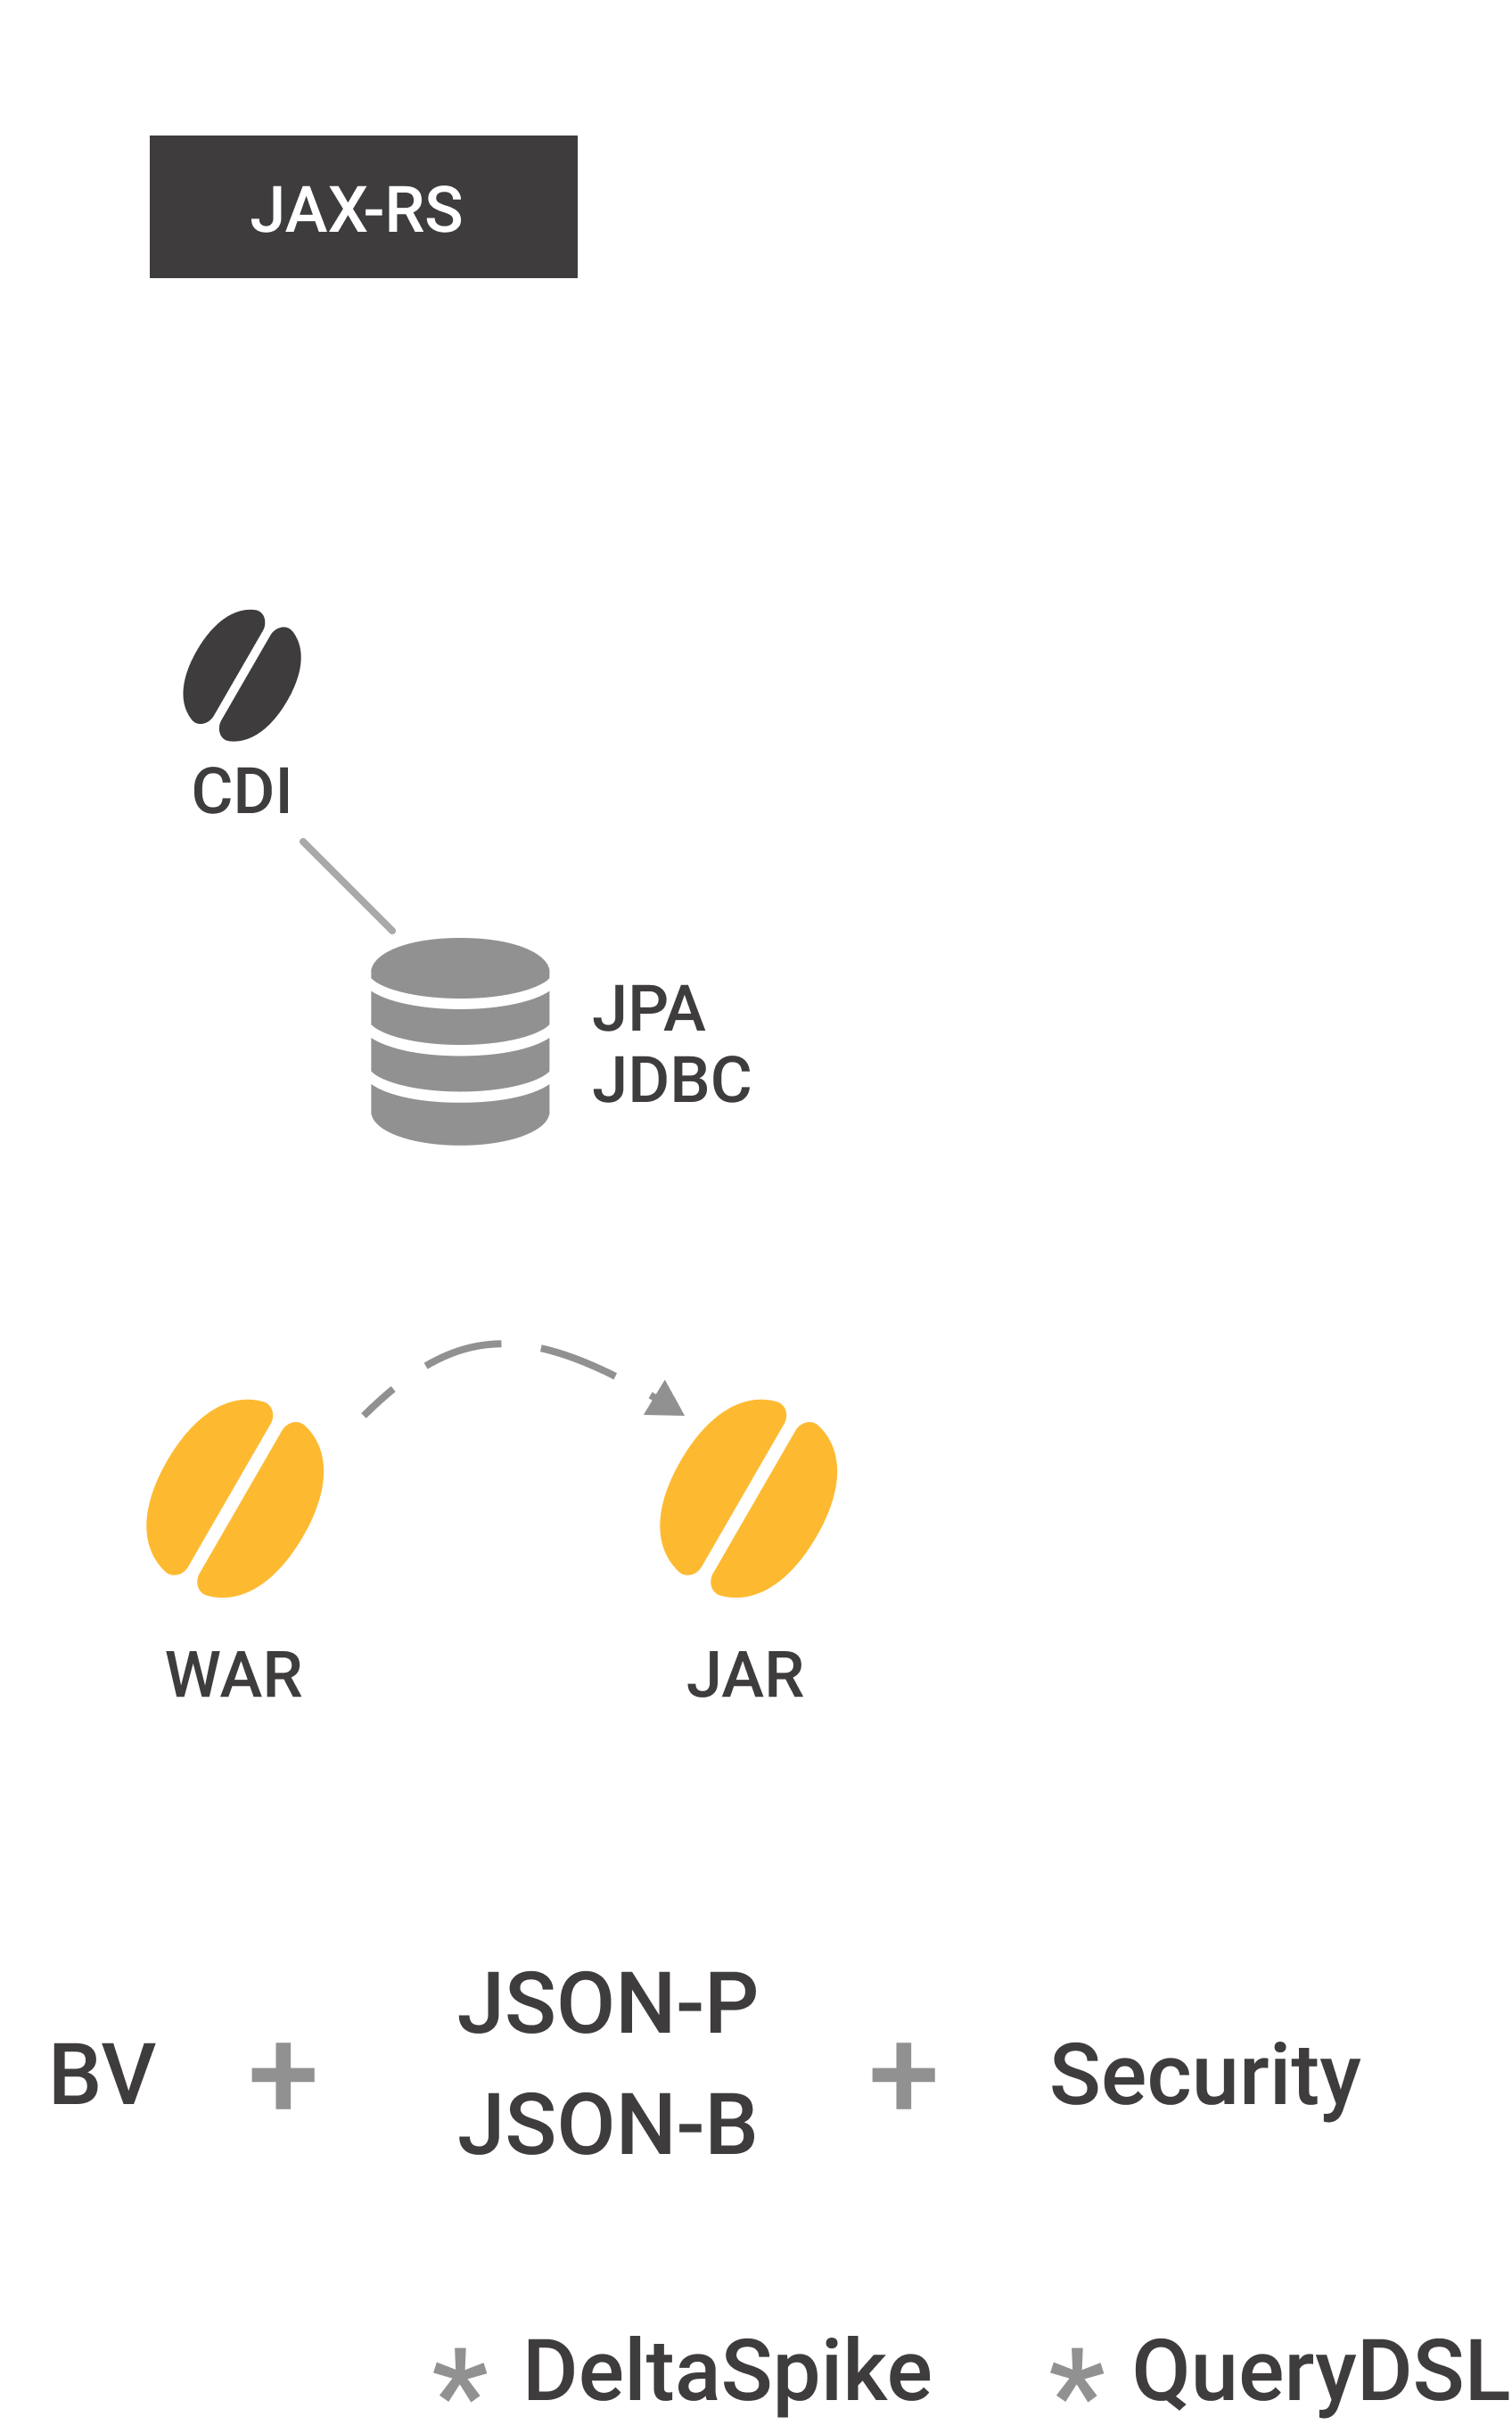
\includegraphics[width=0.4\linewidth]{Images/newsetup}
\end{figure}
\end{frame}

\begin{frame}{Eclipse MicroProfile}
\begin{figure}
	\centering
	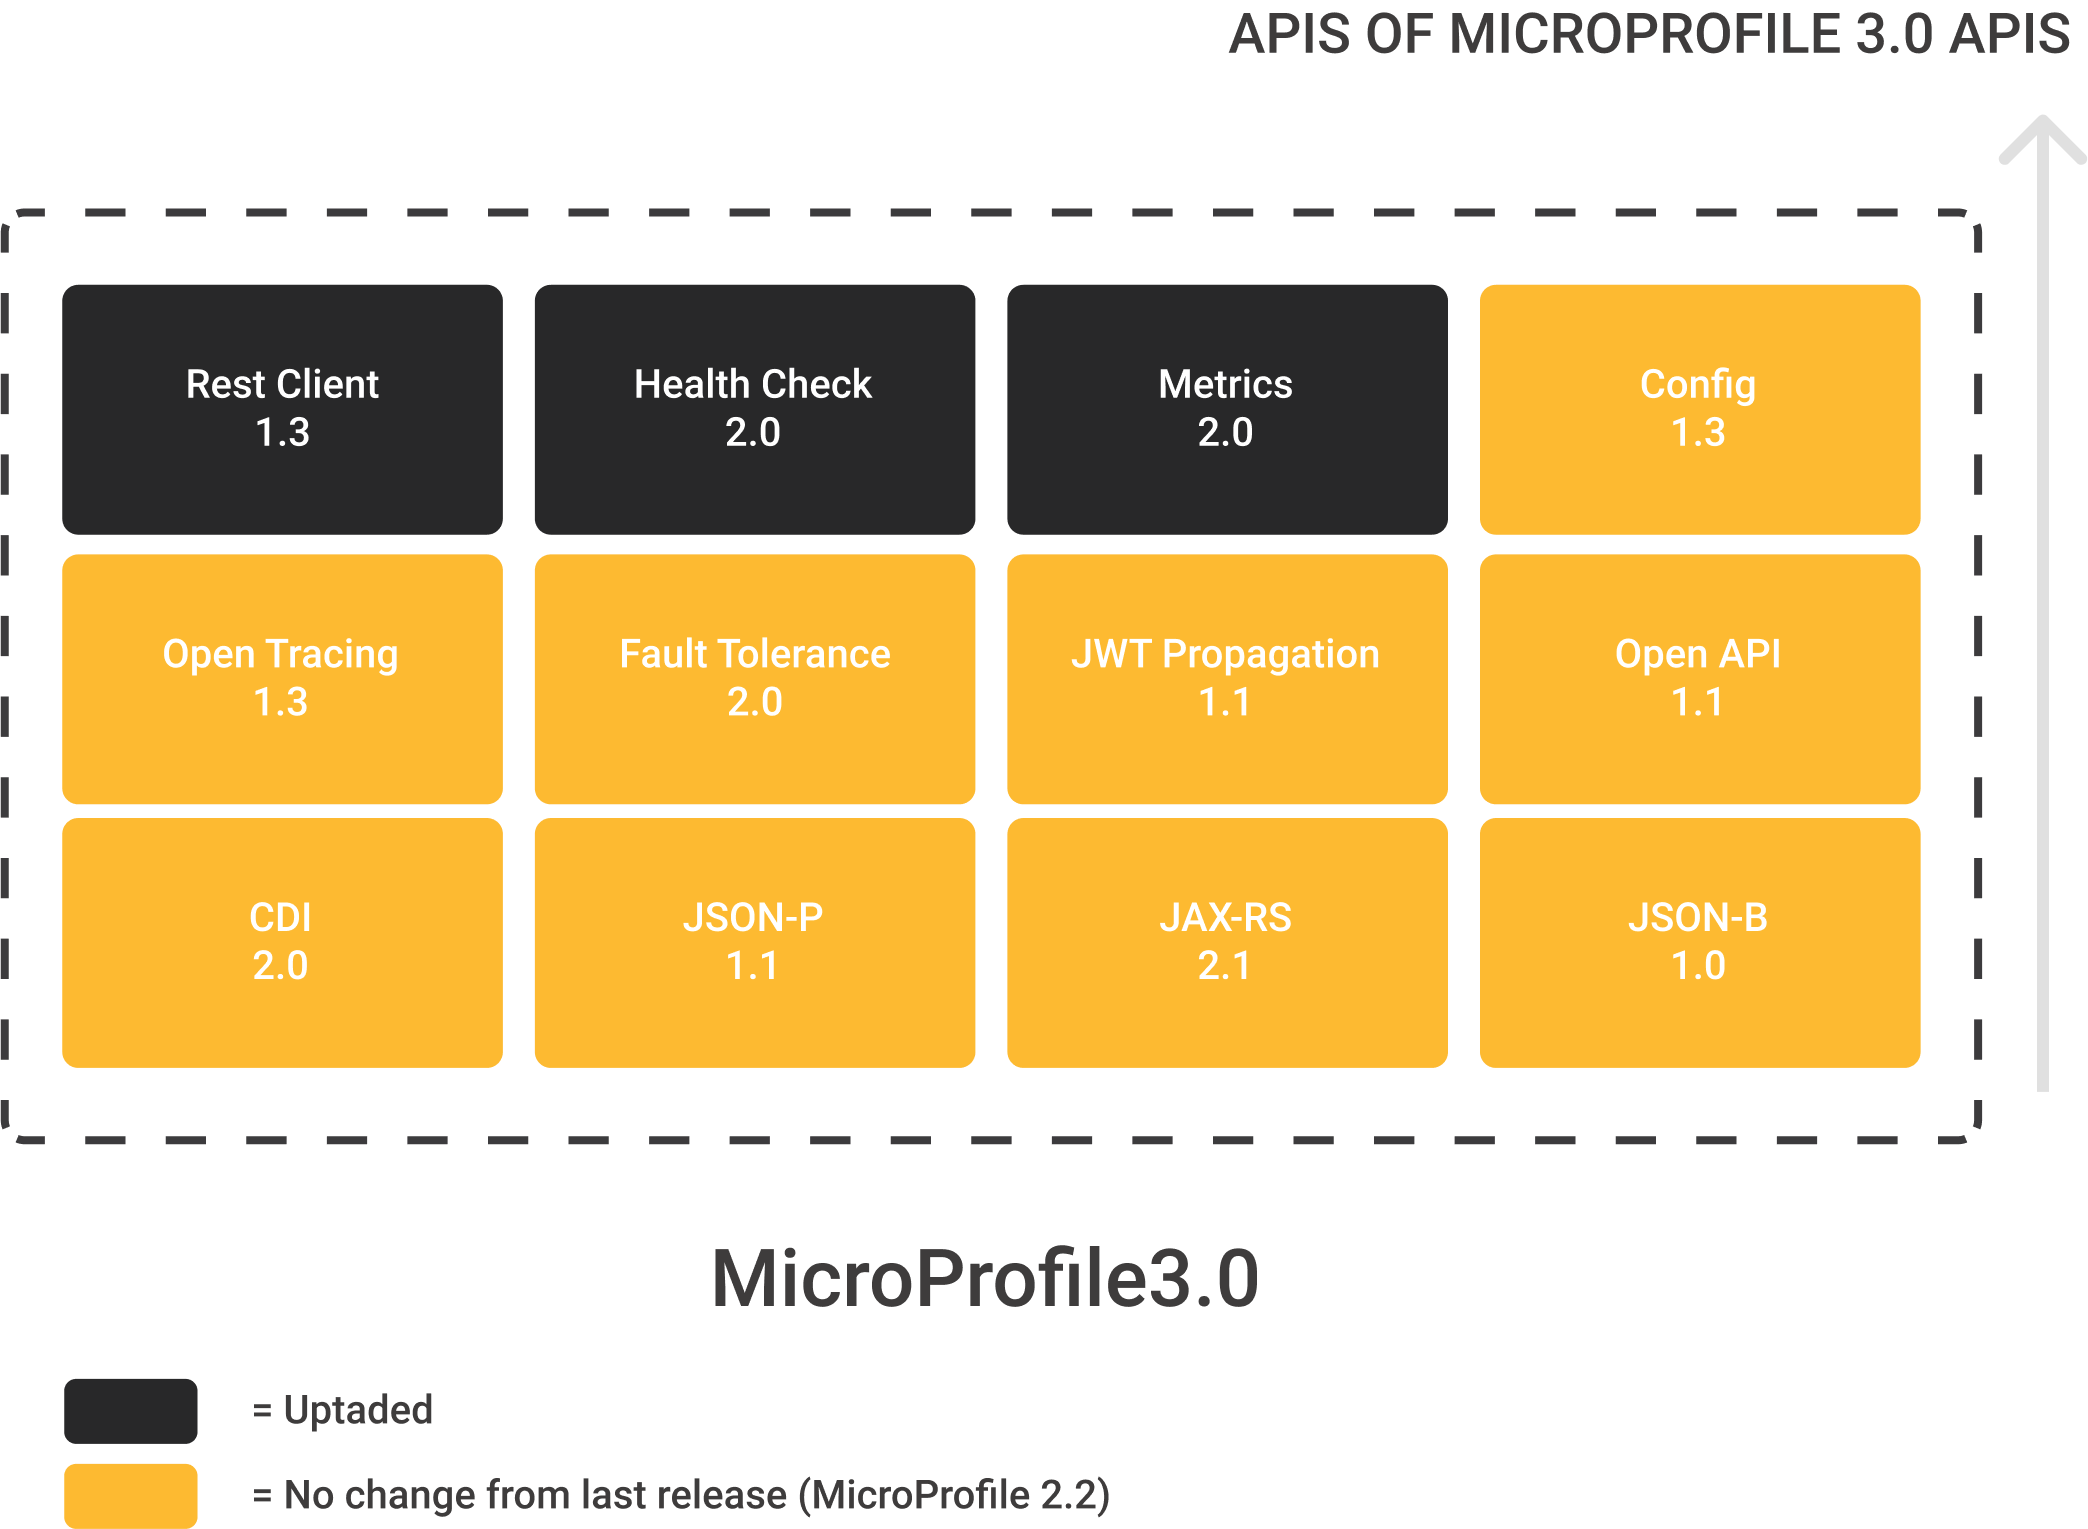
\includegraphics[width=0.9\linewidth]{Images/microprofileapis}
\end{figure}
\end{frame}

%TODO 12 fatores

\begin{frame}{Eclipse MicroProfile - Implementaciones}

Bibliotecas
\begin{itemize}
	\item SmallRye (Red Hat)
	\item Hammock
	\item Apache Geronimo
	\item Fujitsu Launcher
\end{itemize}

JEAS - Fat Jar
\begin{itemize}
	\item Dropwizard
	\item KumuluzEE
	\item Helidon (Oracle)
	\item Open Liberty (IBM)
	\item Quarkus (Red Hat)
\end{itemize}

\end{frame}
\begin{frame}{Eclipse MicroProfile - Implementaciones}

Micro server
\begin{itemize}
	\item Payara Micro
	\item TomEE MicroProfile
\end{itemize}

Full server
\begin{itemize}
	\item Payara Application Server
    \item Apache TomEE
	\item JBoss Application Server / Wildfly Application Server
	\item WebSphere Liberty (IBM)
\end{itemize}

https://wiki.eclipse.org/MicroProfile/Implementation
\end{frame}

{
    \usebackgroundtemplate{
\includegraphics[width=\paperwidth]{Images/separador}}
    \setbeamercolor{normal text}{fg=white}
    \setbeamercolor{frametitle}{fg=red}
    \usebeamercolor[fg]{normal text}
    \section{Eclipse MicroProfile - Objetivos}
}

\begin{frame}[fragile]{Eclipse MicroProfile en Payara 5}
\LARGE Demo MicroProfile Starter
\end{frame}

\begin{frame}{Eclipse MicroProfile}
\begin{figure}
	\centering
	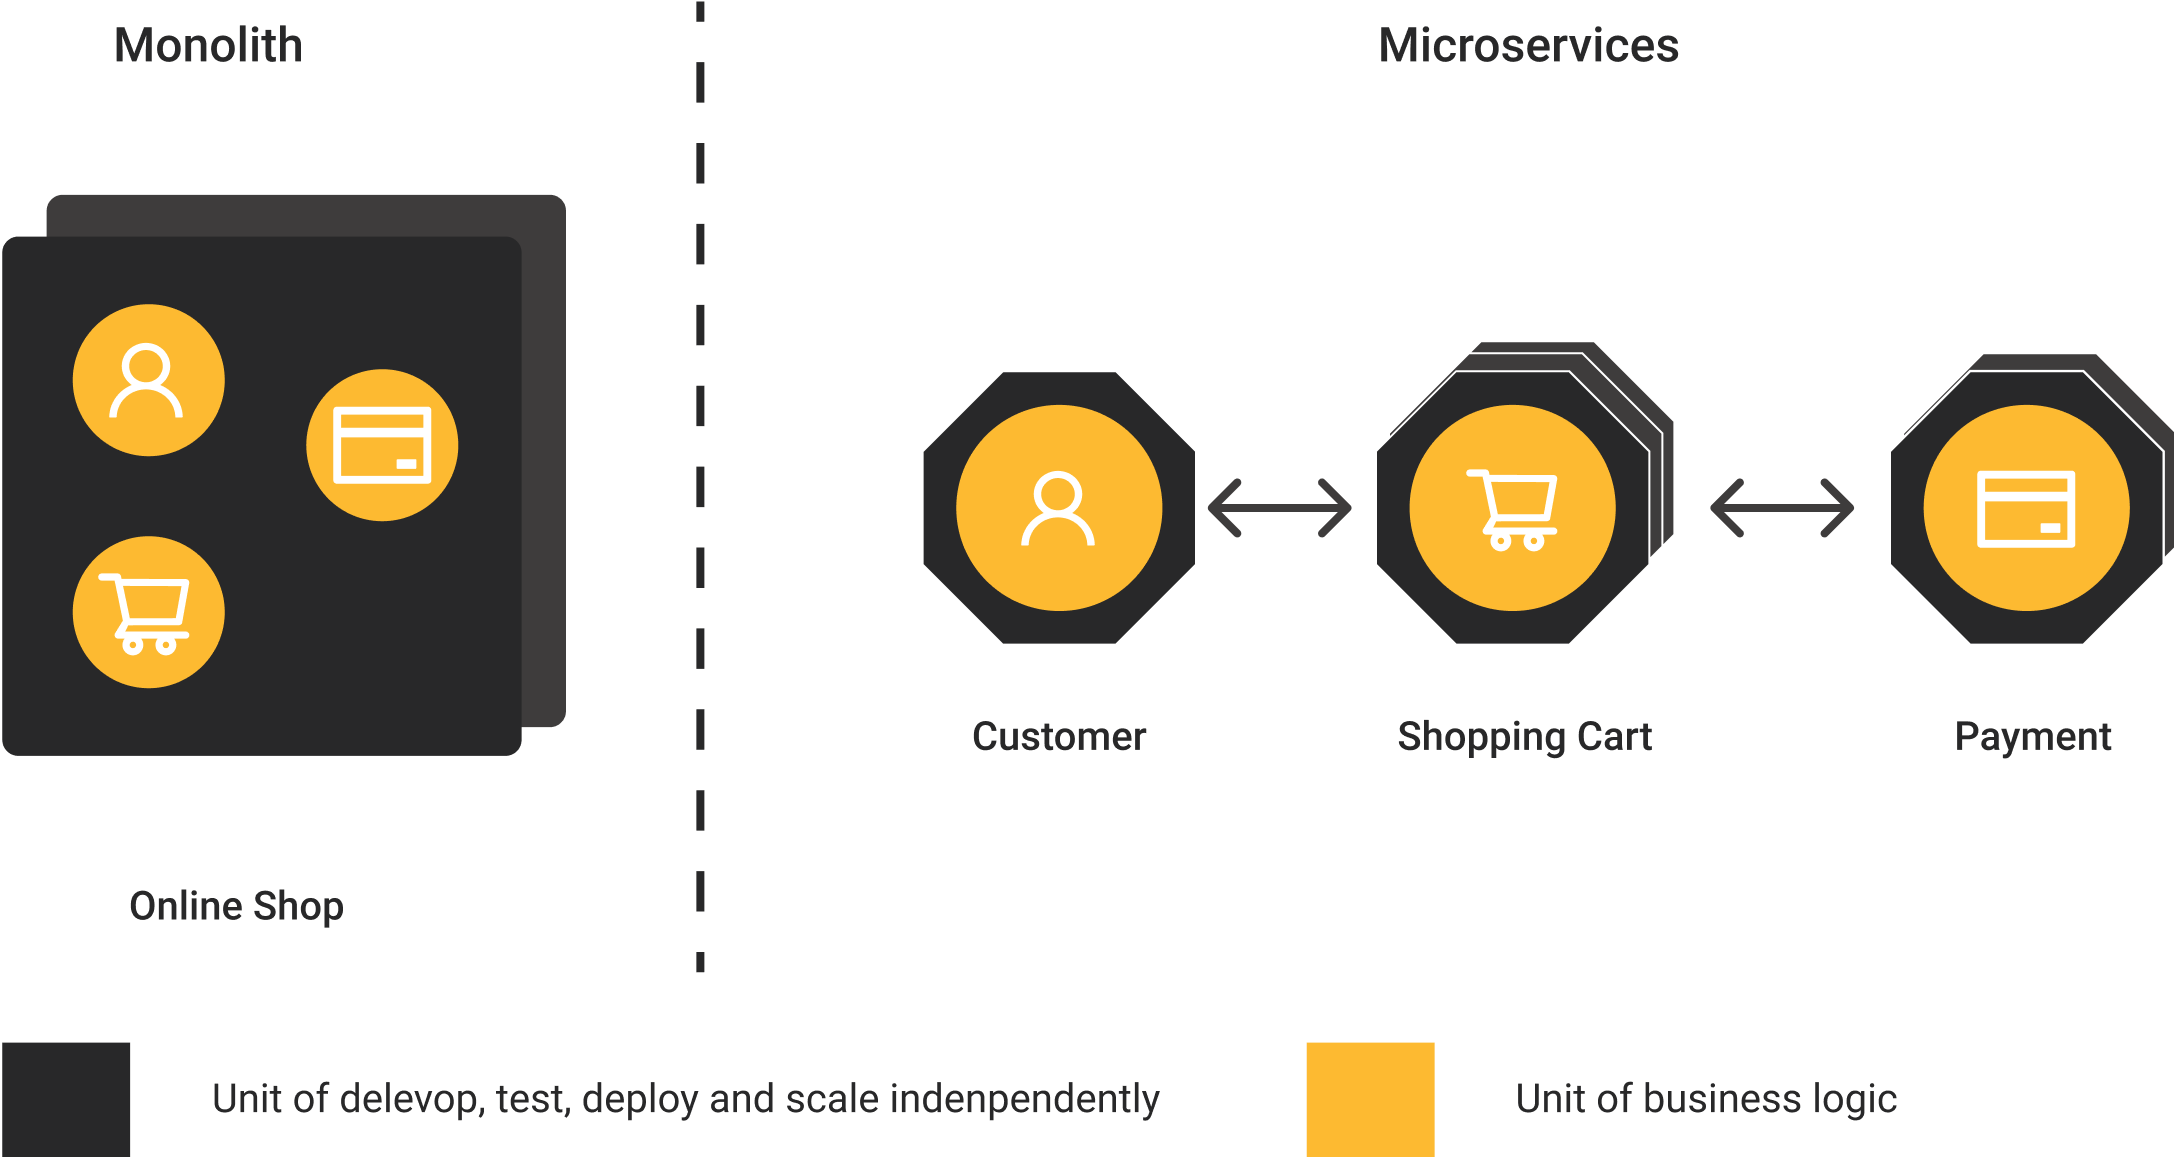
\includegraphics[width=0.8\linewidth]{Images/mp0}
\end{figure}
\end{frame}

\begin{frame}{Eclipse MicroProfile - Coreografia}
\begin{figure}
	\centering
	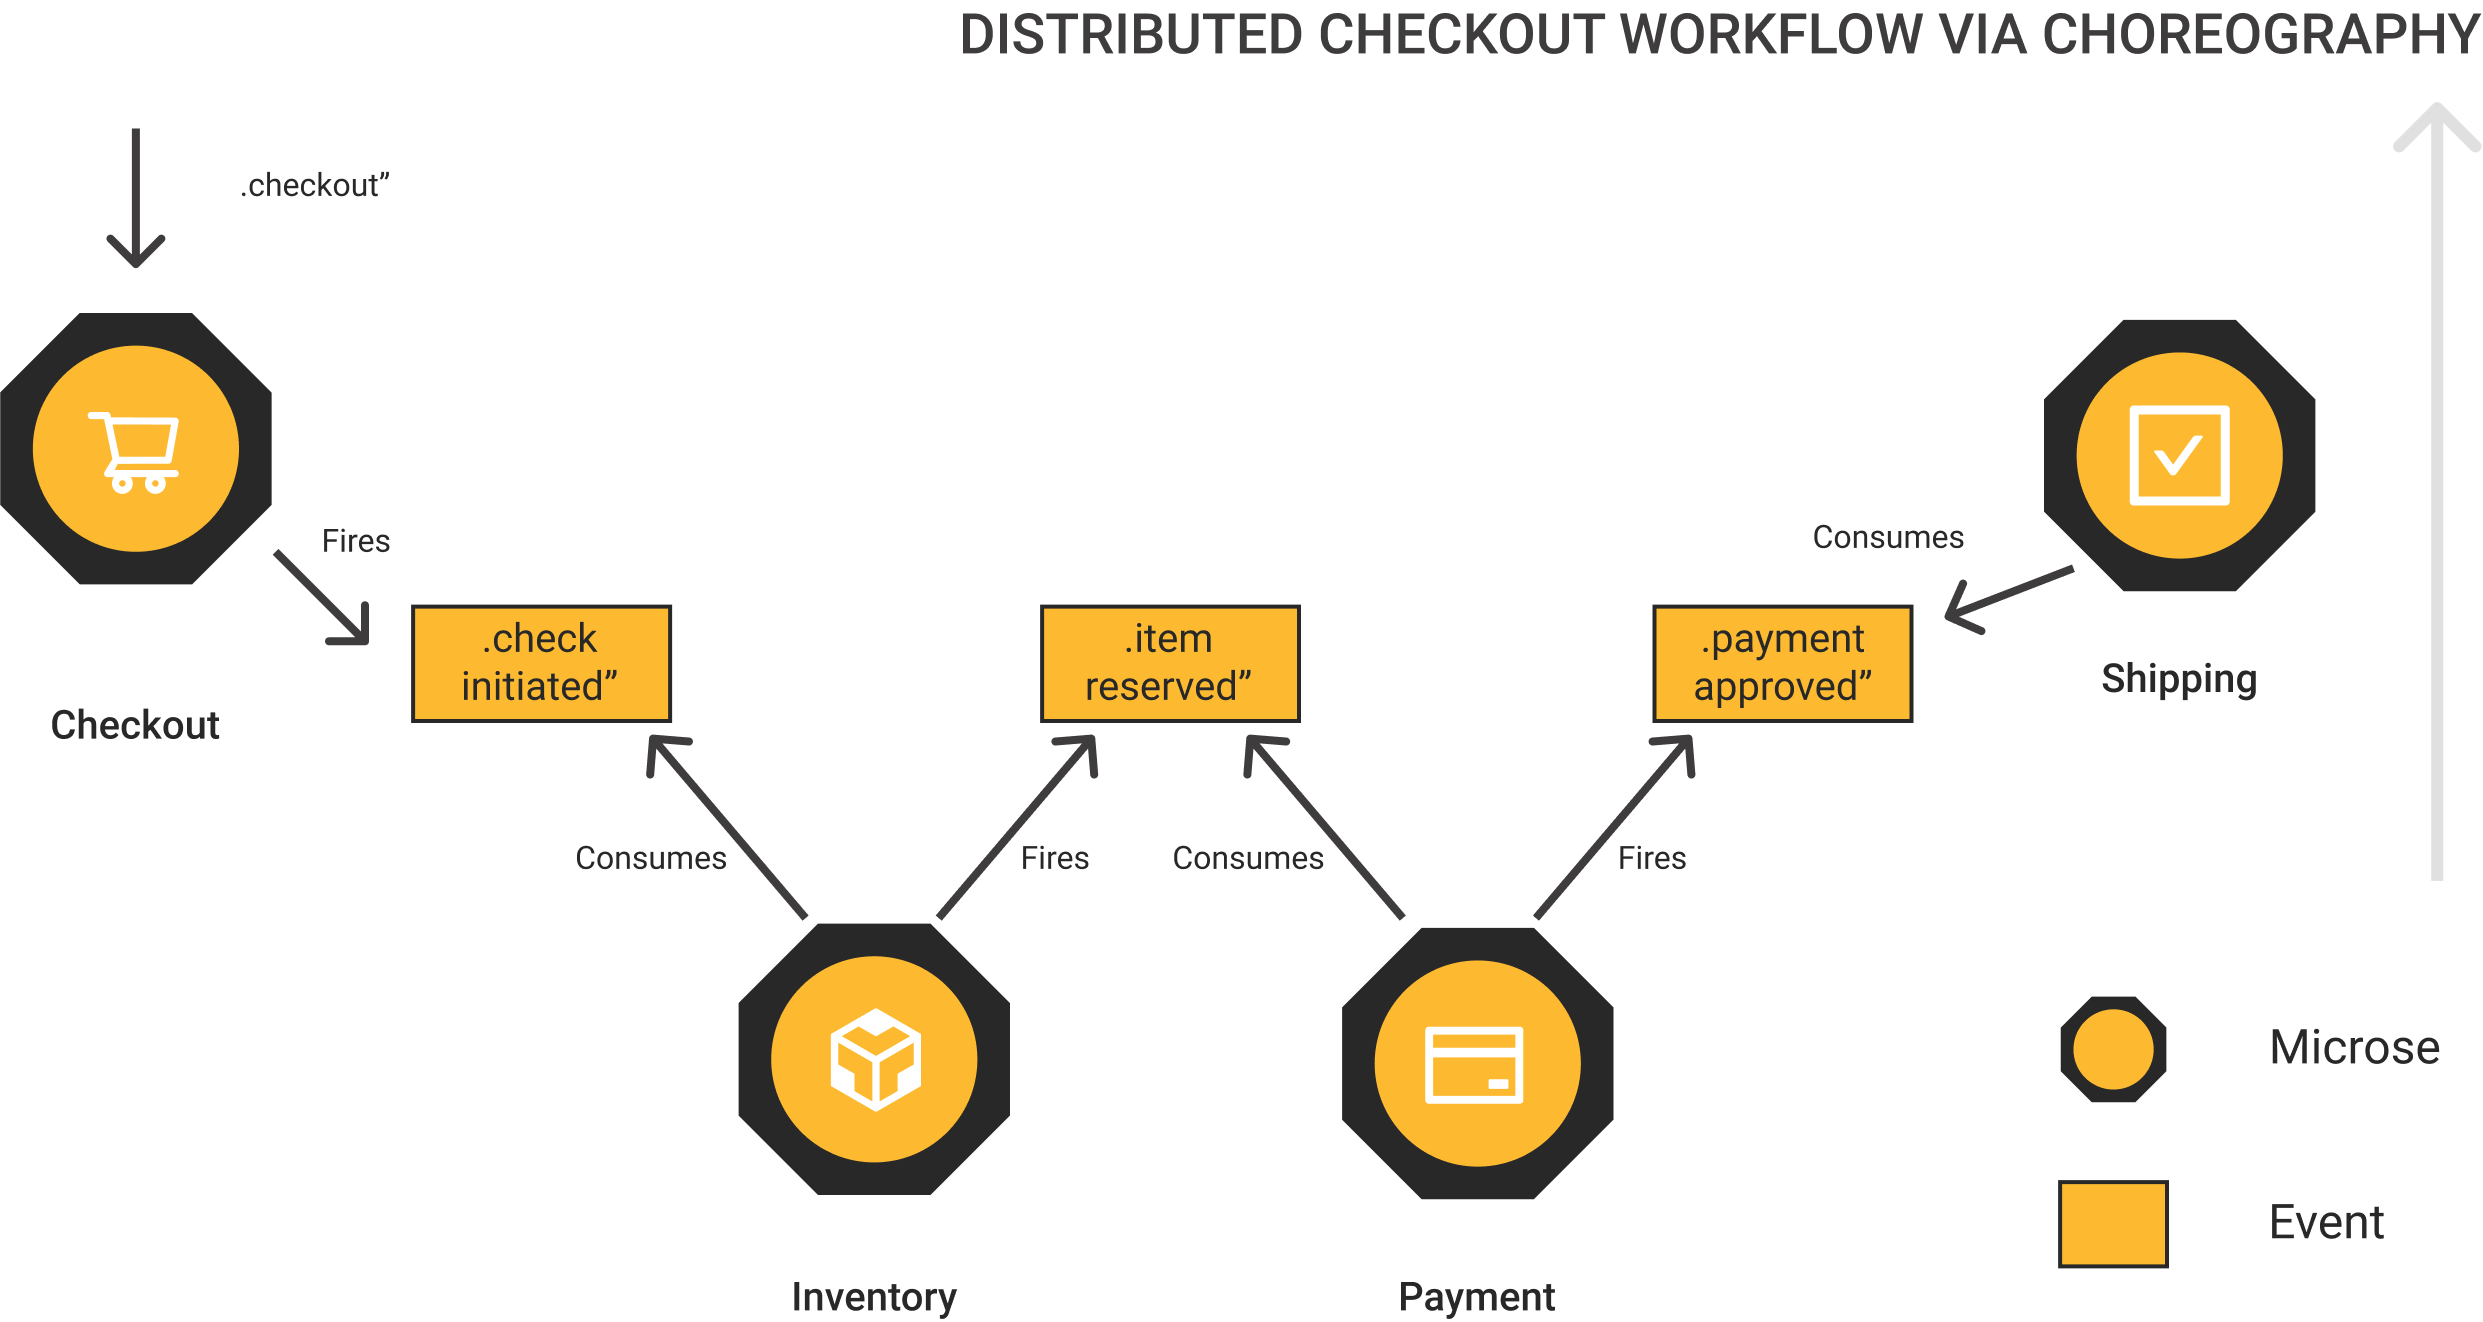
\includegraphics[width=0.8\linewidth]{Images/mpcore}
\end{figure}
\end{frame}

\begin{frame}{Eclipse MicroProfile - Orquestación}
\begin{figure}
	\centering
	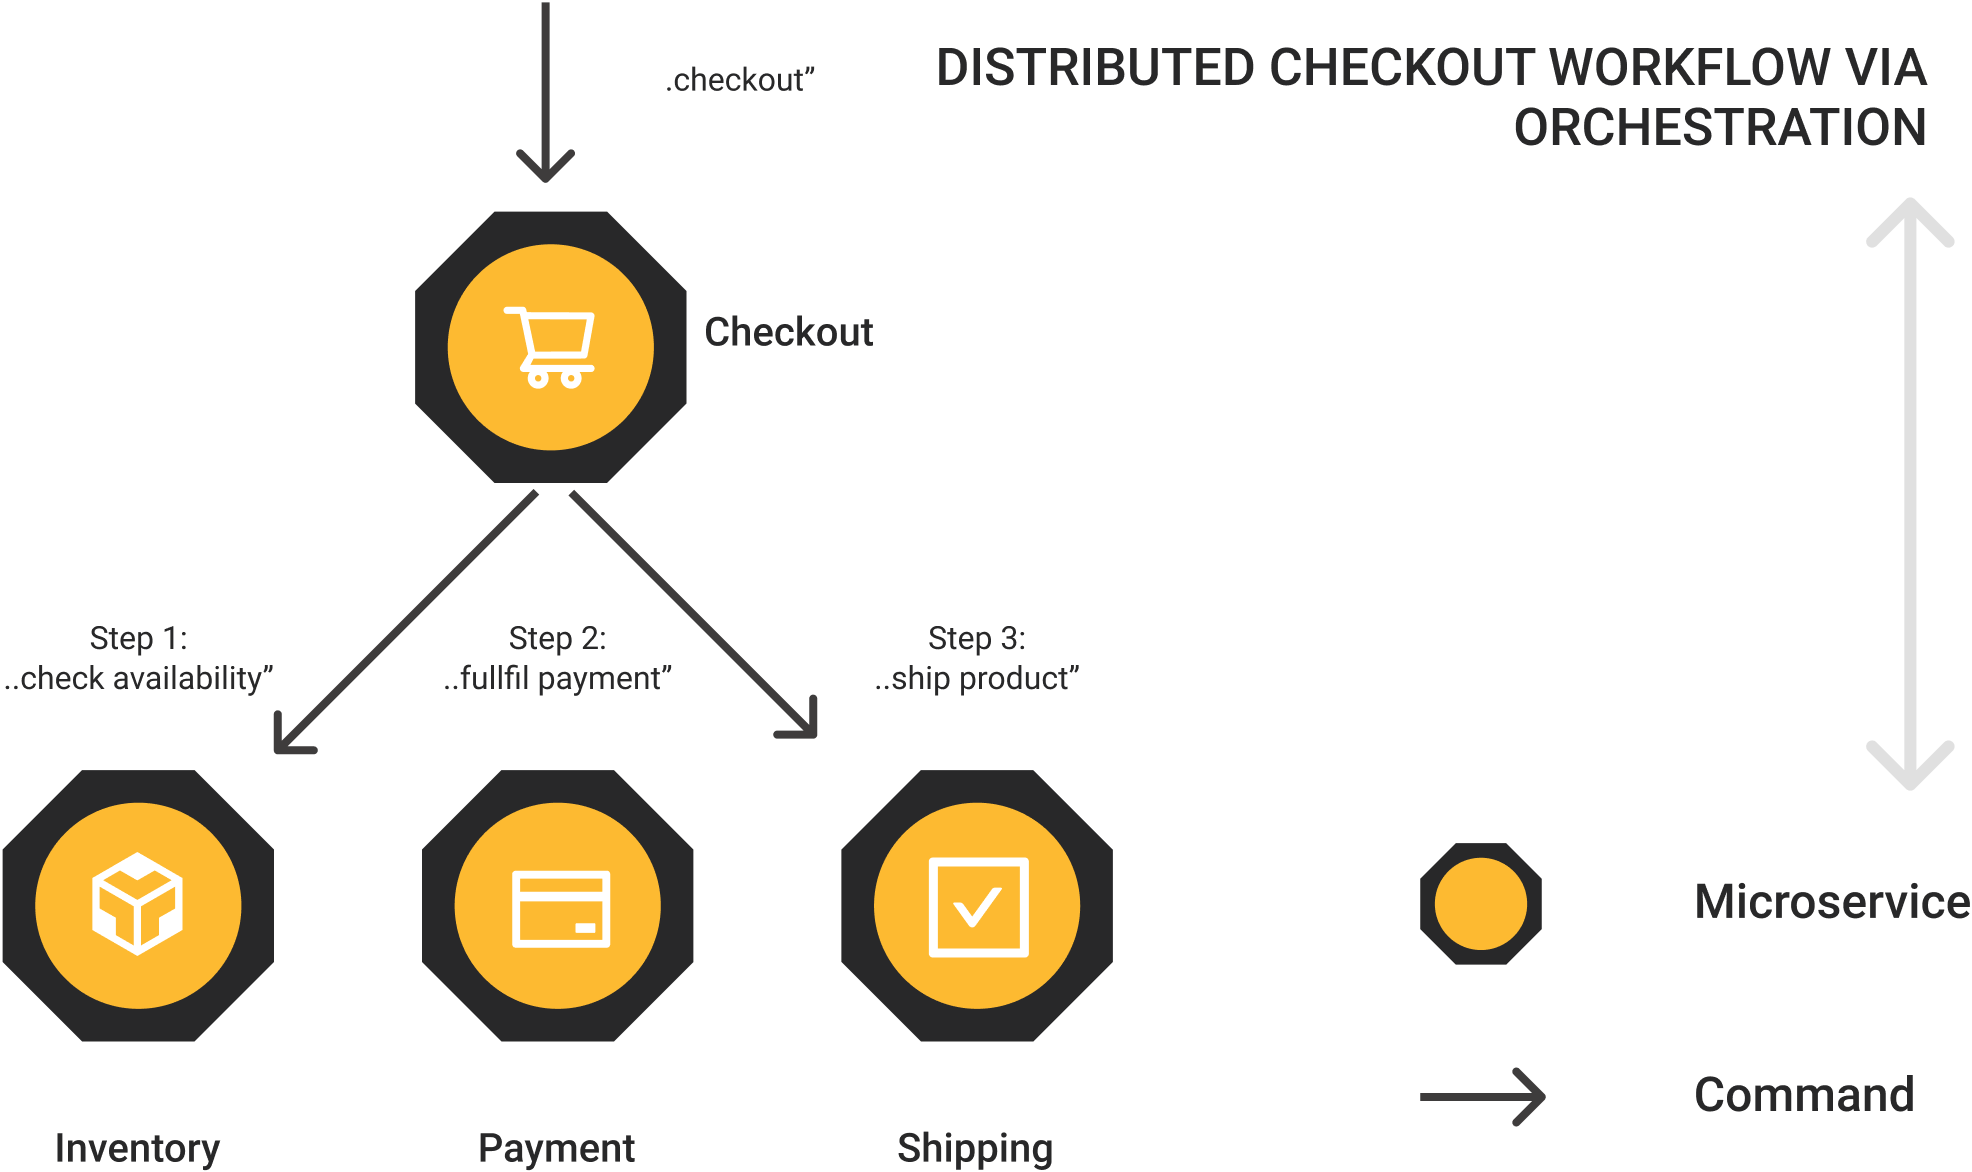
\includegraphics[width=0.8\linewidth]{Images/mporch}
\end{figure}
\end{frame}

\begin{frame}{Eclipse MicroProfile - Cross-cutting concerns}

\begin{itemize}
	\item Health checks \& Metrics
	\item Resilence \& Fault Tolerance
	\item Configuration
	\item Authentication \& Authorization
	\item Standarized documentation
    \item Tracing
\end{itemize}

\end{frame}


{
    \usebackgroundtemplate{
\includegraphics[width=\paperwidth]{Images/separador}}
    \setbeamercolor{normal text}{fg=white}
    \setbeamercolor{frametitle}{fg=red}
    \usebeamercolor[fg]{normal text}
    \section{Eclipse MicroProfile - APIs}
}

\begin{frame}{Config}
\begin{figure}
	\centering
	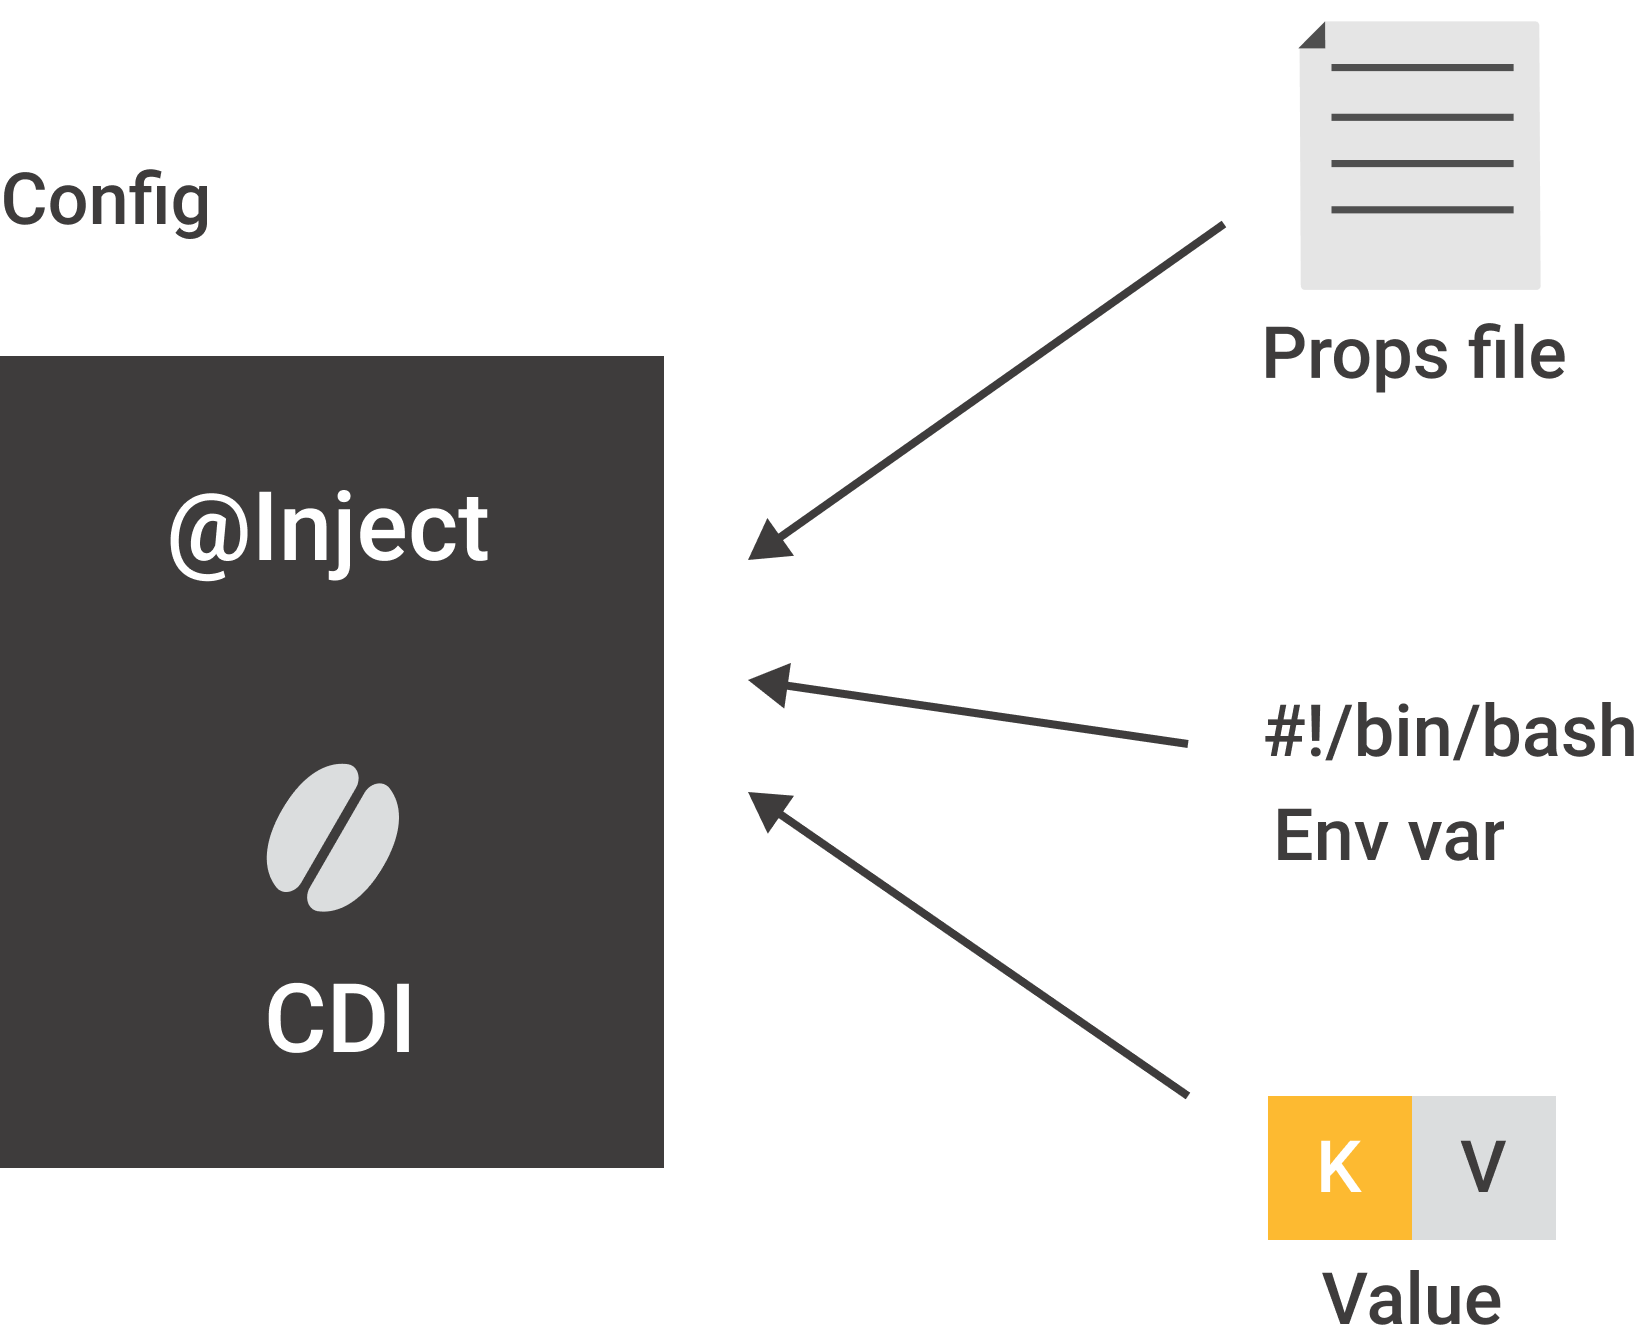
\includegraphics[width=0.65\linewidth]{Images/config}
\end{figure}
\end{frame}

\begin{frame}{Config}
\begin{figure}
	\centering
	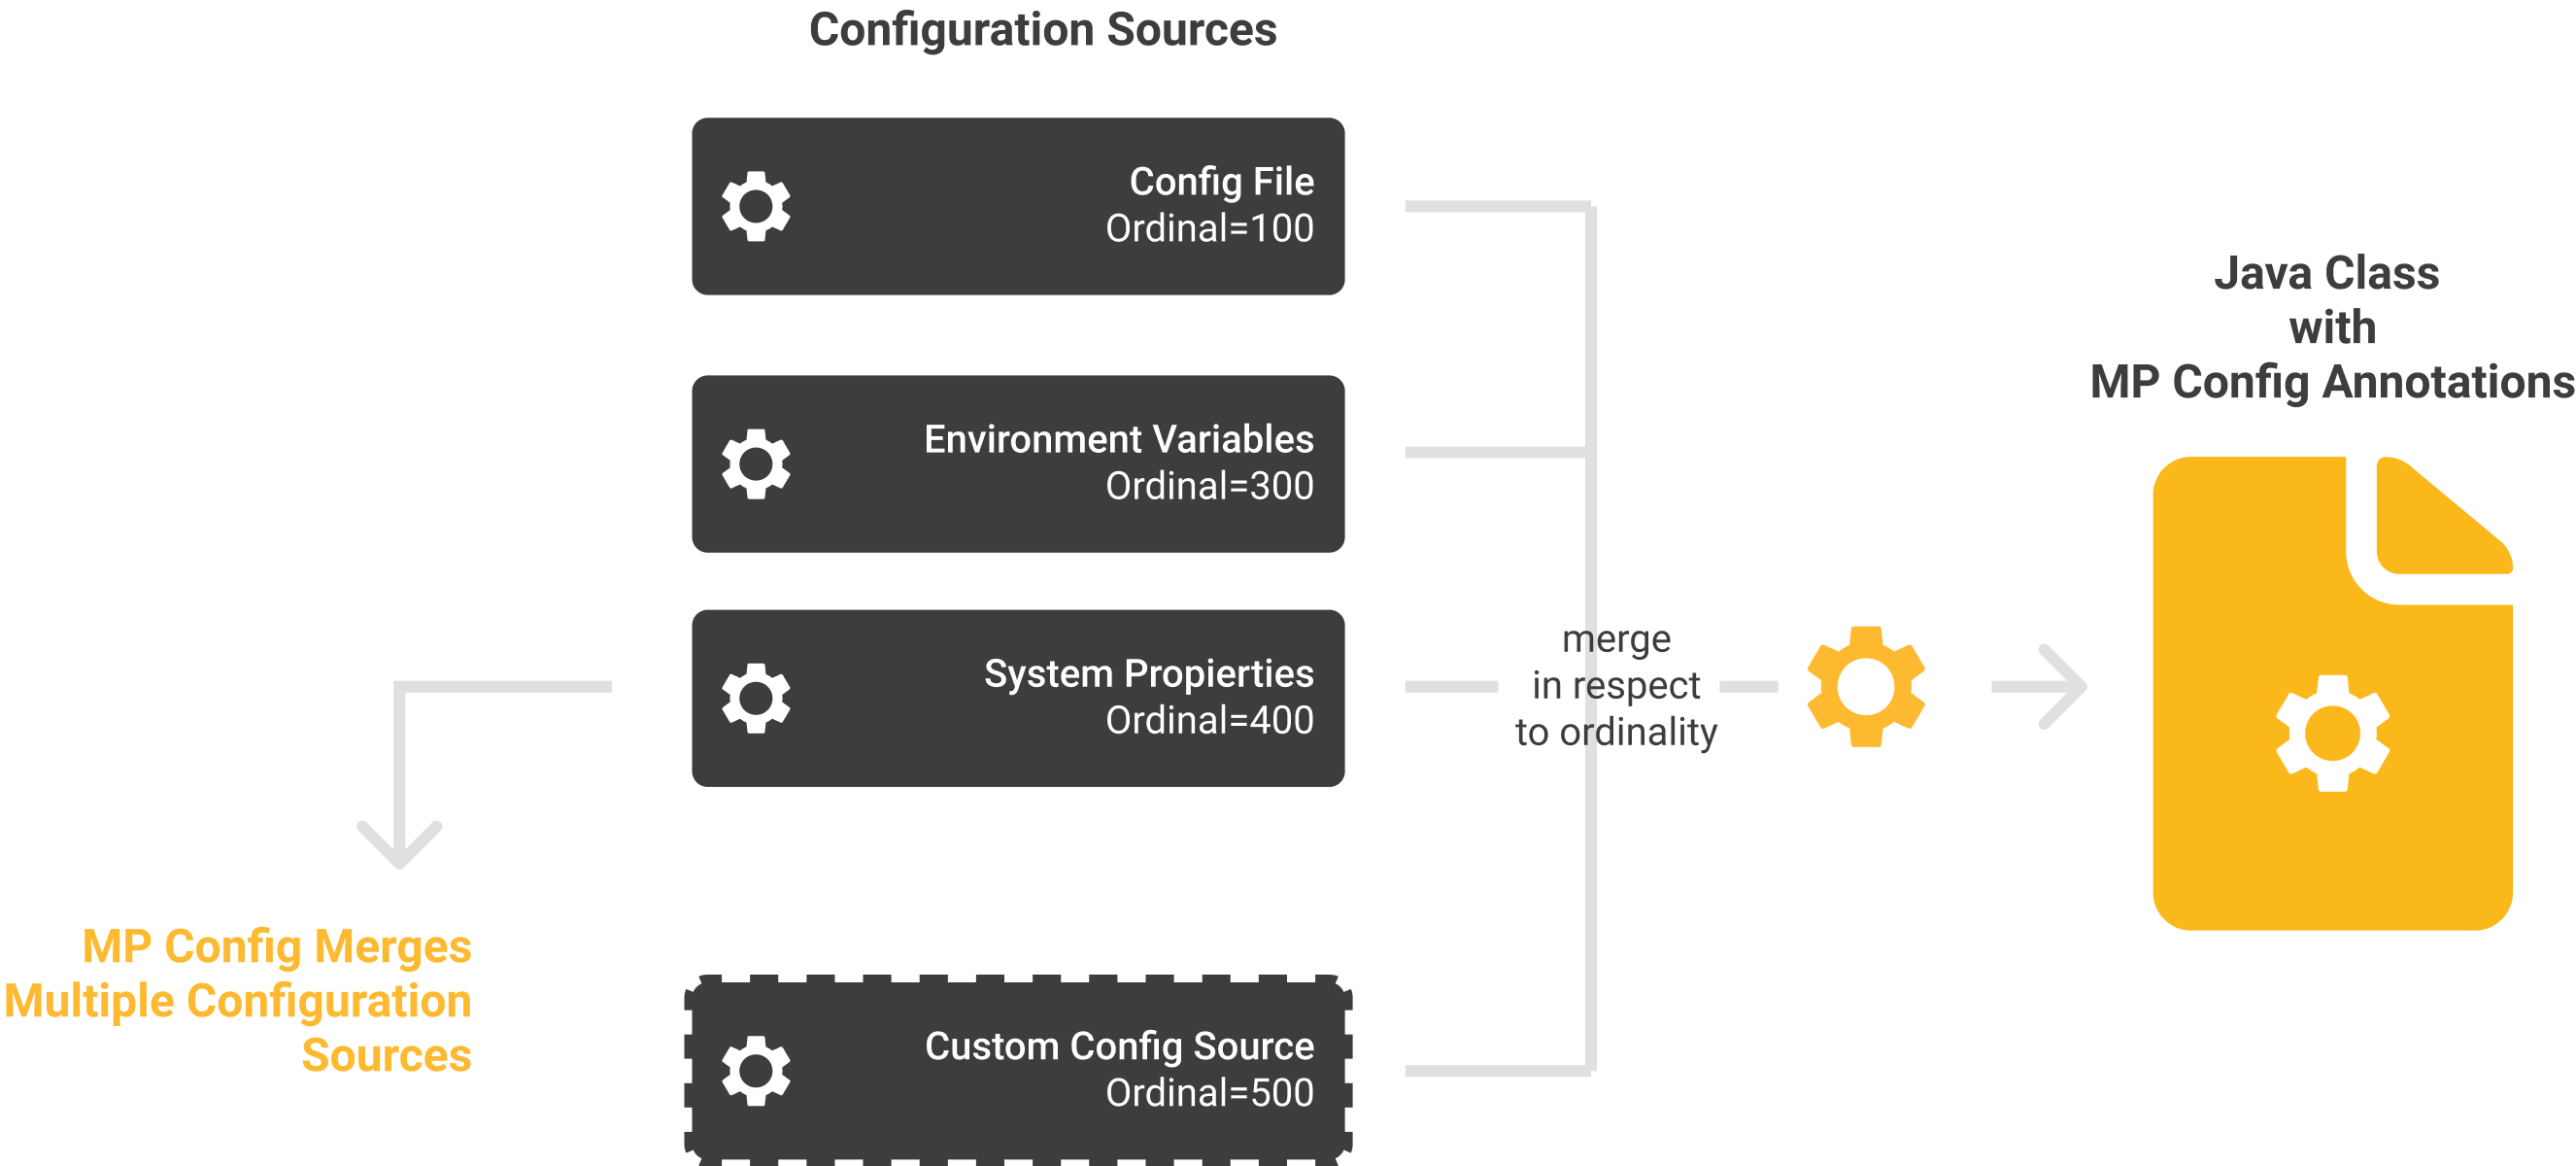
\includegraphics[width=0.8\linewidth]{Images/mpconfig}
\end{figure}
\end{frame}




\begin{frame}[fragile]{Config}
\begin{lstlisting}
@Inject
<@\textcolor{red}{@ConfigProperty(name = "omdbservice.url")}@>
String omdbDaemonServiceUrl;
\end{lstlisting}

Ext. de la configuración (VM, Docker, Kubernetes)
\end{frame}



\begin{frame}[fragile]{Config}
\begin{lstlisting}
@Inject
@ConfigProperty(name = "application.currency")
private String currency;

@Inject
@ConfigProperty(name = "application.list.maxSize",
	defaultValue="10")
private Integer maxSize;
\end{lstlisting}
\end{frame}

\begin{frame}[fragile]{Config}
No CDI, no hay problema
\begin{lstlisting}
final Config config = ConfigProvider.getConfig();
config.getValue("application.curreny", String.class);
config.getOptionalValue("application.list.maxSize",
	Integer.class);
\end{lstlisting}
\end{frame}

\begin{frame}[fragile]{Config}
Propiedades dinámicas
\begin{lstlisting}
@Inject @ConfigProperty(name="userId")
Provider<String> userId;
\end{lstlisting}
\end{frame}

\begin{frame}[fragile]{Config}
Inyección global
\begin{lstlisting}
@Inject Config config;
\end{lstlisting}
\end{frame}

\begin{frame}[fragile]{OpenAPI - Aplicación}
APIs documentadas en formato estandard

\begin{itemize}
	\item @APIResponses - Respuestas multiples de una API
	\item @APIResponse - Respuesta unica de una API
	\item @Content - Esquema y ejemplo
	\item @Schema - I/O data types
	\item @Operation - Describe la operación
	\item @Parameter - Describe el parámetro de una operación
\end{itemize}

\end{frame}

\begin{frame}[fragile]{OpenAPI - Aplicación}
APIs documentadas en formato estandard
\begin{lstlisting}
@ApplicationPath("/api")
@OpenAPIDefinition(info = @Info(
	title = "Example application",
	version = "1.0.0",
	contact = @Contact(
	name = "Victor Orozoc",
	email = "vorozco@nabenik.com",
	url = "http://vorozco.com")
	),
	servers = {
		@Server(url = "/example",
		description = "localhost")
	}
)
public class ApplicationConfig extends Application {
\end{lstlisting}
\end{frame}

\begin{frame}[fragile]{OpenAPI}
APIs documentadas en formato estandard
\begin{lstlisting}
@GET @Path("/{key}")
@Operation(description = "Get the value for this key")
@APIResponses({
	@APIResponse(responseCode = "200",
	description = "Successful, returning the value")
})
@Produces(MediaType.TEXT_PLAIN)
public Response getConfigValue(@PathParam("key") String key)
\end{lstlisting}
\end{frame}

\begin{frame}{OpenAPI}
\begin{figure}
	\centering
	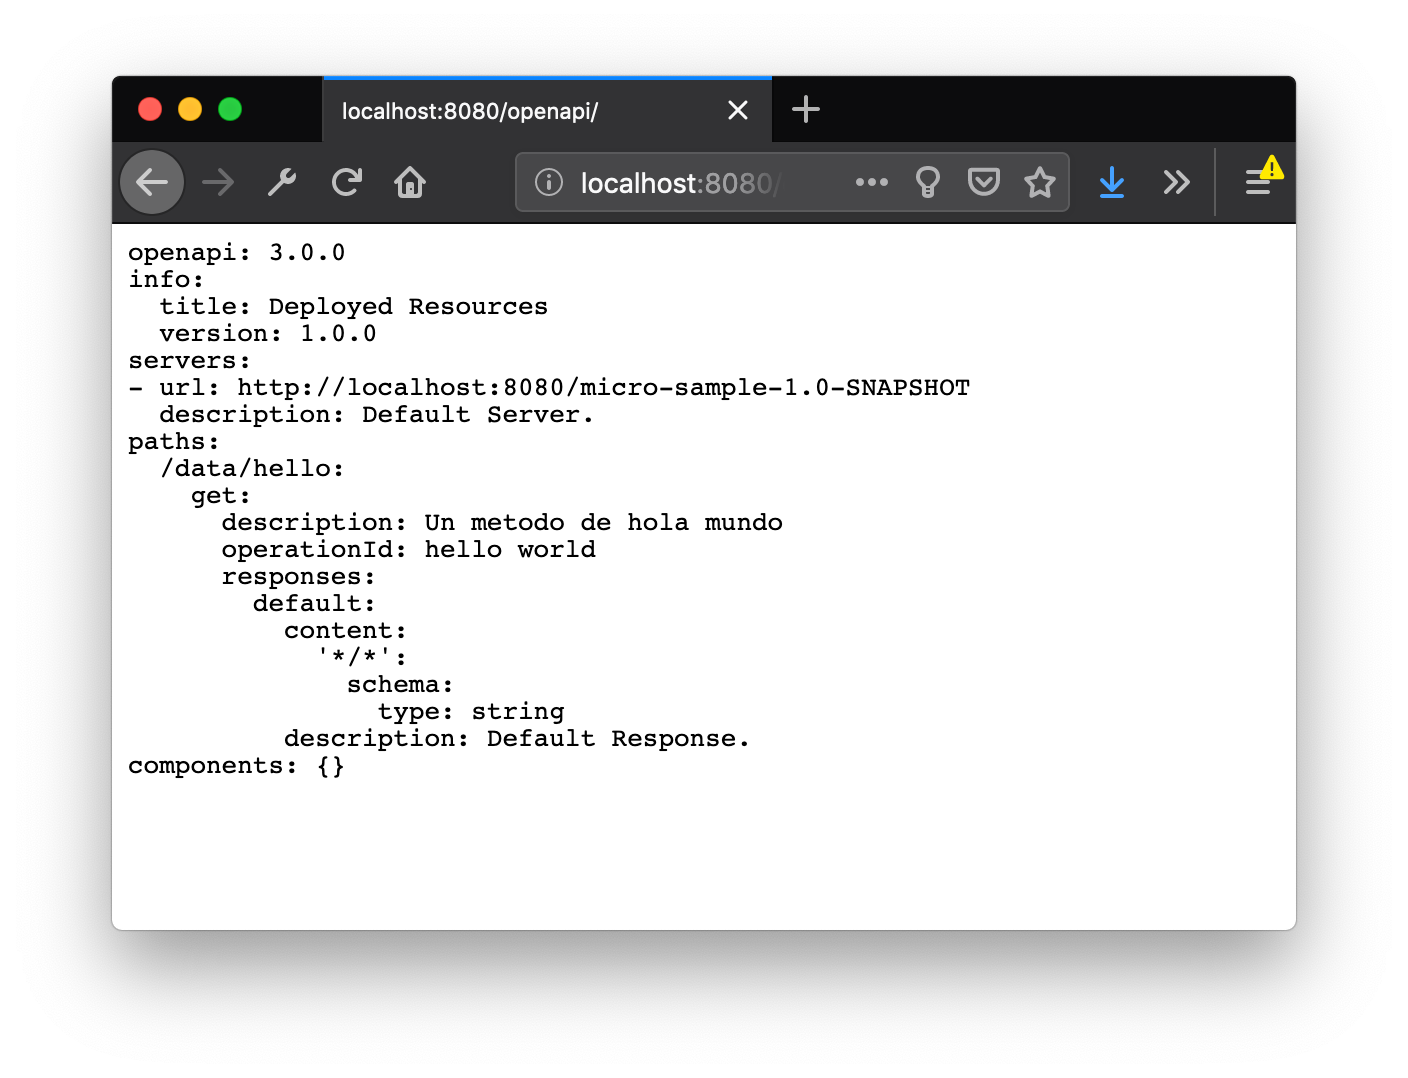
\includegraphics[width=0.75\linewidth]{Images/openapi}
\end{figure}
\end{frame}

\begin{frame}[fragile]{OpenAPI - Swagger UI}
APIs documentadas en formato estandard
\begin{lstlisting}
<dependency>
	<groupId>org.microprofile-ext.openapi-ext</groupId>
	<artifactId>swagger-ui</artifactId>
	<version>1.0.2</version>
</dependency>
\end{lstlisting}
\end{frame}

\begin{frame}{Fault Tolerance}
\begin{figure}
	\centering
	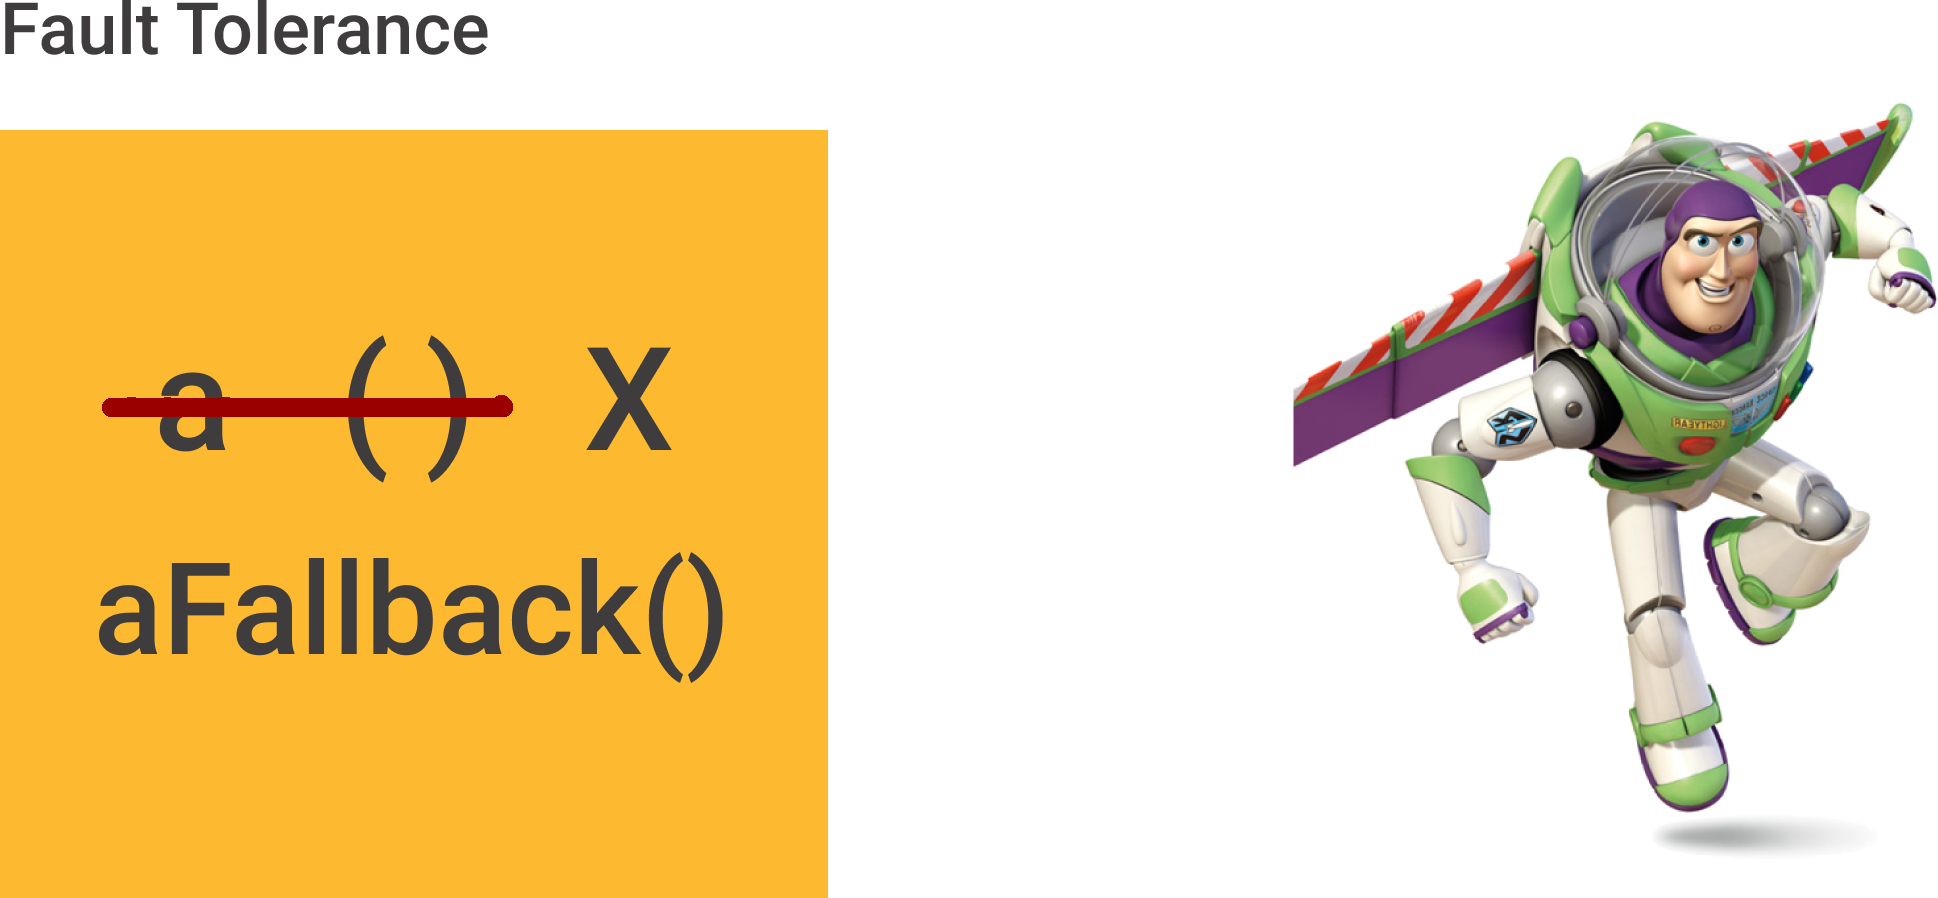
\includegraphics[width=0.75\linewidth]{Images/faulttolerance}
\end{figure}
\end{frame}

\begin{frame}{Metrics}
\begin{figure}
	\centering
	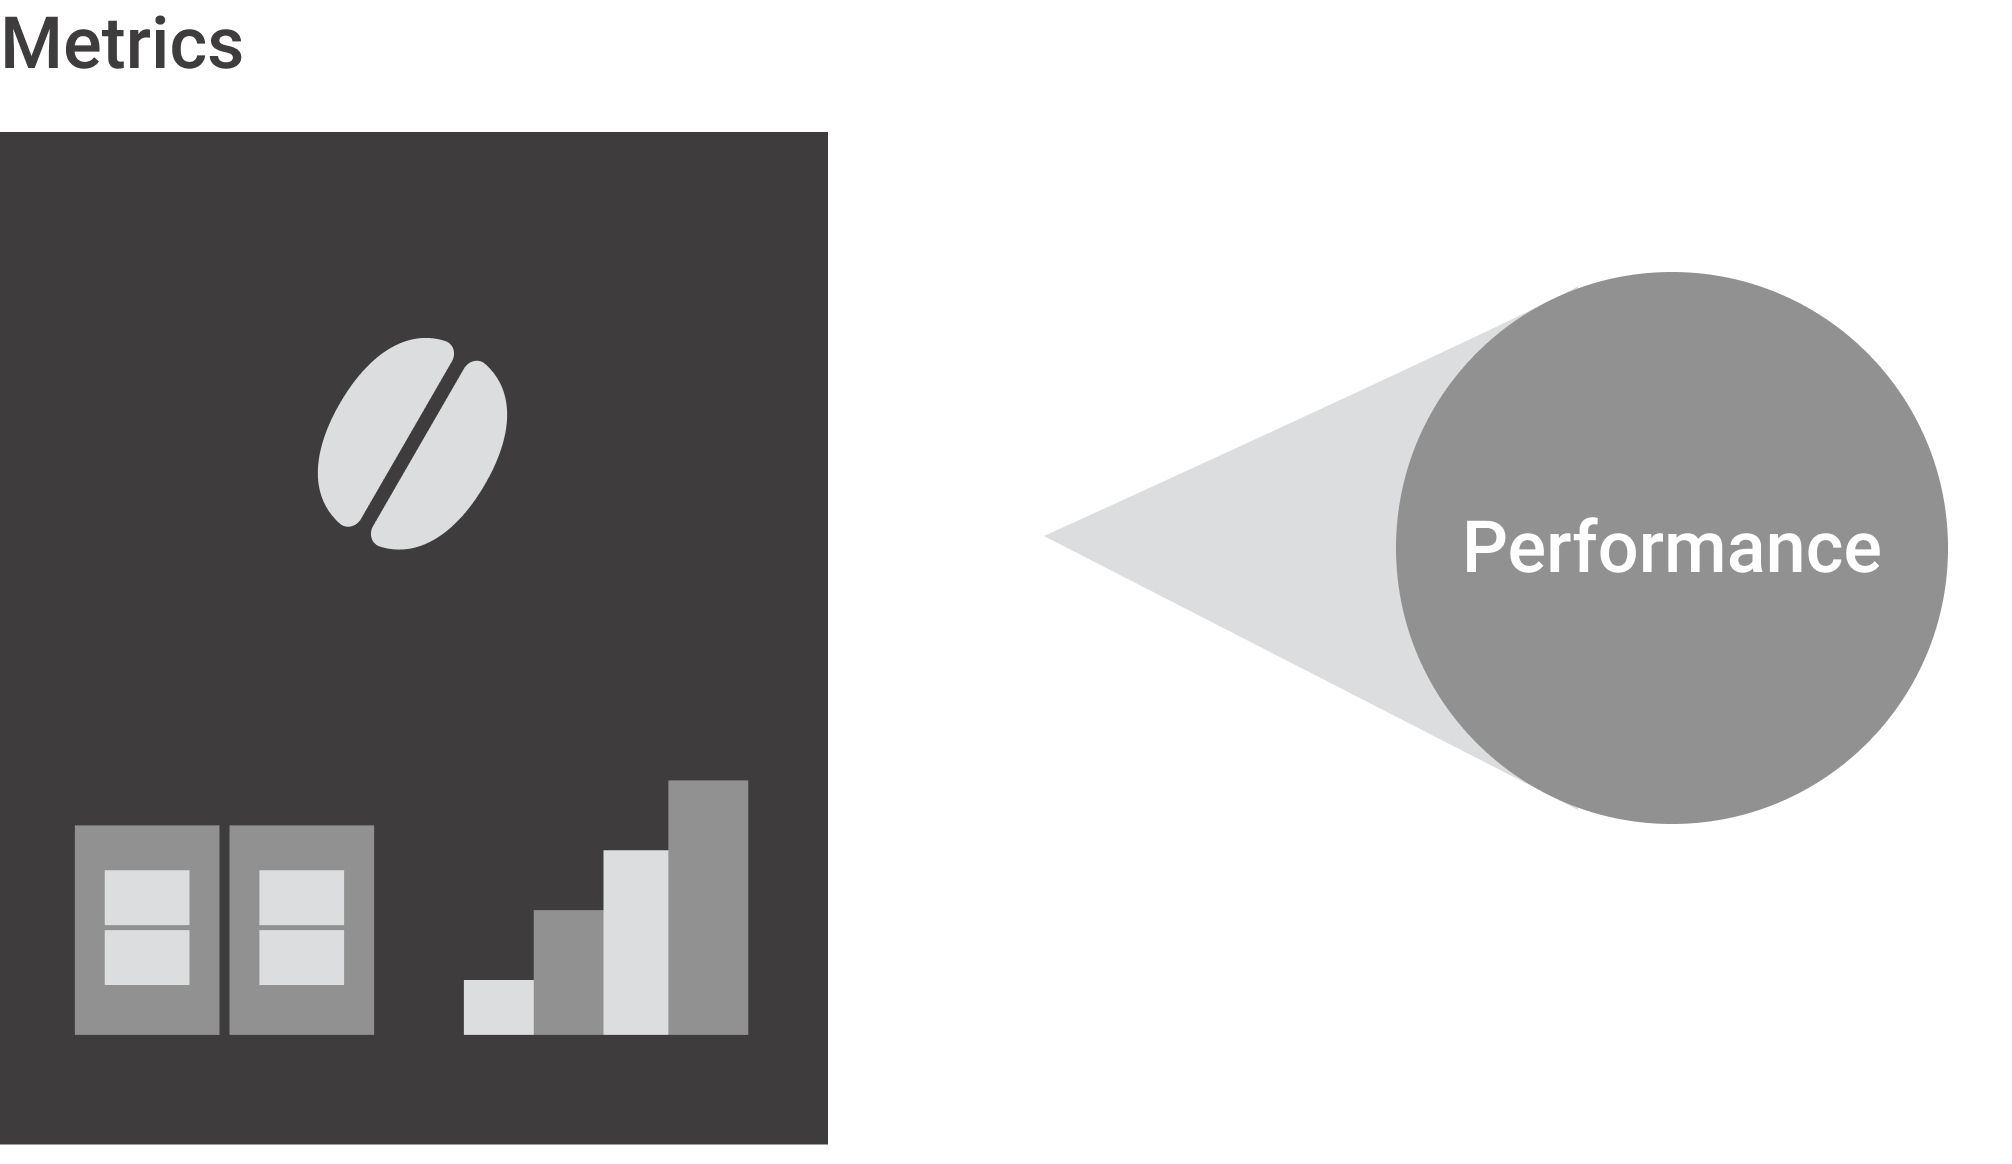
\includegraphics[width=0.75\linewidth]{Images/metrics}
\end{figure}
\end{frame}




\begin{frame}{Fault Tolerance + Metrics}

\begin{itemize}
	\item \textit{Fault Tolerance} depende de la existencia de metricas, las metricas se exponen  mediante \textit{Metrics}
\end{itemize}

\begin{figure}
	\centering
	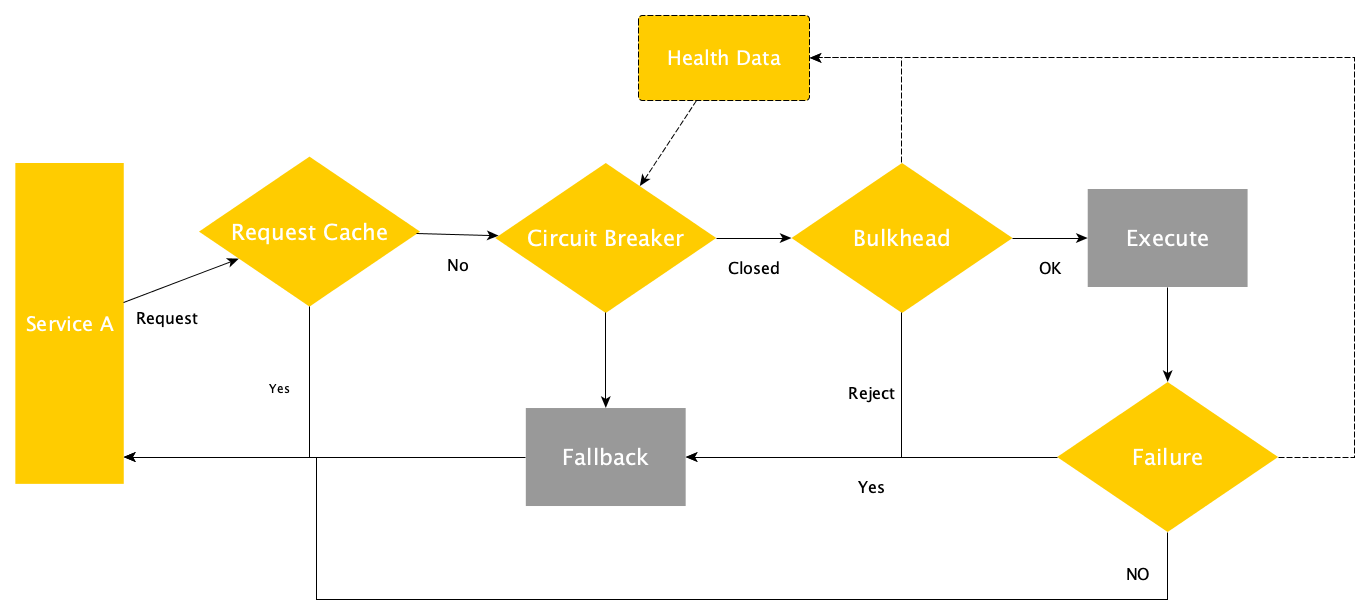
\includegraphics[width=0.9\linewidth]{Images/falldata}
\end{figure}

\end{frame}


\begin{frame}{Fault tolerance}

Reglas de evaluación y alternativas
\begin{itemize}
\item Circuit Breaker
\item Bulkhead
\item Retry
\item Timeout
\item Fallback
\end{itemize}

\end{frame}

\begin{frame}[fragile]{Fault tolerance - Retry}
\begin{lstlisting}
@Retry(delay = 400, maxDuration= 3200, jitter= 400, maxRetries = 10)
public Connection serviceA() {
	...
}

@Retry(retryOn = {IOException.class})
public void serviceB() {
	...
}
\end{lstlisting}
\end{frame}

\begin{frame}[fragile]{Fault tolerance - CircuitBreaker}
\begin{lstlisting}
@CircuitBreaker(successThreshold = 10,
	requestVolumeThreshold = 4,
	failureRatio=0.75,
	delay = 1000)
public Connection serviceA() {
	Connection conn = null;
	conn = connectionService();
	return conn;
}
\end{lstlisting}
\end{frame}

\begin{frame}[fragile]{Fault tolerance - Bulkhead}
\begin{lstlisting}
@Bulkhead(5)
public Connection serviceA() {
	Connection conn = null;
	conn = connectionService();
	return conn;
}
\end{lstlisting}

\begin{lstlisting}
@Asynchronous
@Bulkhead(value = 5, waitingTaskQueue = 8)
public Future<Connection> serviceA() {
	Connection conn = null;
	conn = connectionService();
	return CompletableFuture.completedFuture(conn);
}

\end{lstlisting}
\end{frame}



\begin{frame}[fragile]{Fault tolerance - Fallback, Timeout}
\begin{lstlisting}
@GET
@Path("/{id:[a-z]*[0-9][0-9]*}")
<@\textcolor{red}{@Fallback(fallbackMethod = "findByIdFallBack")}@>
<@\textcolor{red}{@Timeout(TIMEOUT)}@>
public Response findById(@PathParam("id")
final String imdbId) {
...
}

public Response findByIdFallBack(@PathParam("id")
final String imdbId) {
...
}
\end{lstlisting}
\end{frame}

\begin{frame}[fragile]{Fault tolerance - Fallback Handler, Timeout}
\begin{lstlisting}
@GET
@Path("/{id:[a-z]*[0-9][0-9]*}")
<@\textcolor{red}{@Fallback(MovieFindAllFallbackHandler.class)}@>
<@\textcolor{red}{@Timeout(TIMEOUT)}@>
public Response findById(@PathParam("id")
final String imdbId) {
...
}
\end{lstlisting}
\begin{lstlisting}
public class MovieFindAllFallbackHandler
	implements FallbackHandler<List> {
	@Override
	public List handle(final ExecutionContext context) {
		return Stream.of("Star Wars",
		"The Matrix", "Cantinflas").collect(toList());
	}
}
\end{lstlisting}
\end{frame}


\begin{frame}{Métricas}

\begin{itemize}
	\item JSON or OpenMetrics (Prometheus)
	\item Vendor
	\item Base
	\item Application
\end{itemize}

¿Cuales?
\begin{itemize}
	\item Counted
	\item Gauge
	\item Metered
	\item Timed
	\item Histogram
\end{itemize}

\end{frame}

\begin{frame}[fragile]{Metrics - Counted}
\begin{lstlisting}
@Inject
<@\textcolor{red}{@Metric}@>
Counter failedQueries;
\end{lstlisting}

\begin{lstlisting}
@GET
@Path("/{id:[a-z]*[0-9][0-9]*}")
<@\textcolor{red}{@Fallback(fallbackMethod = "findByIdFallBack")}@>
<@\textcolor{red}{@Timeout(TIMEOUT)}@>
public Response findById(@PathParam("id")
final String imdbId) {
...
}

public Response findByIdFallBack(@PathParam("id")
final String imdbId) {
	...
	<@\textcolor{red}{failedQueries.inc();}@>
}
\end{lstlisting}
\end{frame}

\begin{frame}[fragile]{Metrics - Gauge}
Inc-dec en tiempo real
\begin{lstlisting}
<@\textcolor{red}{
@Gauge(unit = "ExternalDatabases",
	name = "movieDatabases", absolute = true)
}@>
public long getDatabases() {
	return 99; //Any value
}
\end{lstlisting}

\lstinline|/metrics/application/movieDatabases|
\end{frame}

\begin{frame}[fragile]{Metrics - Metered}
Events rate
\begin{lstlisting}
@Metered(name = "moviesRetrieved",
	unit = MetricUnits.MINUTES,
	description = "Metrics to monitor movies",
	absolute = true)
public Response findExpandedById(
	@PathParam("id") final Long id)
\end{lstlisting}

\lstinline|/metrics/application/movieDatabases|
\end{frame}

\begin{frame}[fragile]{Metrics- Timed}
Desempeño y retraso
\begin{lstlisting}
@Timed(name = "moviesDelay",
	description = "Time to retrieve a movie",
	unit = MetricUnits.MINUTES,
	absolute = true)
public Response findExpandedById(
	@PathParam("id") final Long id)
\end{lstlisting}

\lstinline|/metrics/application/moviesDelay|
\end{frame}

\begin{frame}[fragile]{Metrics - Histogram}
Distribuciones
\begin{lstlisting}
@Inject
MetricRegistry registry;

@POST
@Path("/add/{attendees}")
public Response addAttendees(
	@PathParam("attendees") Long attendees) {
	Metadata metadata =
		new Metadata("matrix attendees",
			MetricType.HISTOGRAM);
	Histogram histogram =
		registry.histogram(metadata);
	histogram.update(attendees);
	return Response.ok().build();
}
\end{lstlisting}

\end{frame}

\begin{frame}{Health Check}
\begin{figure}
	\centering
	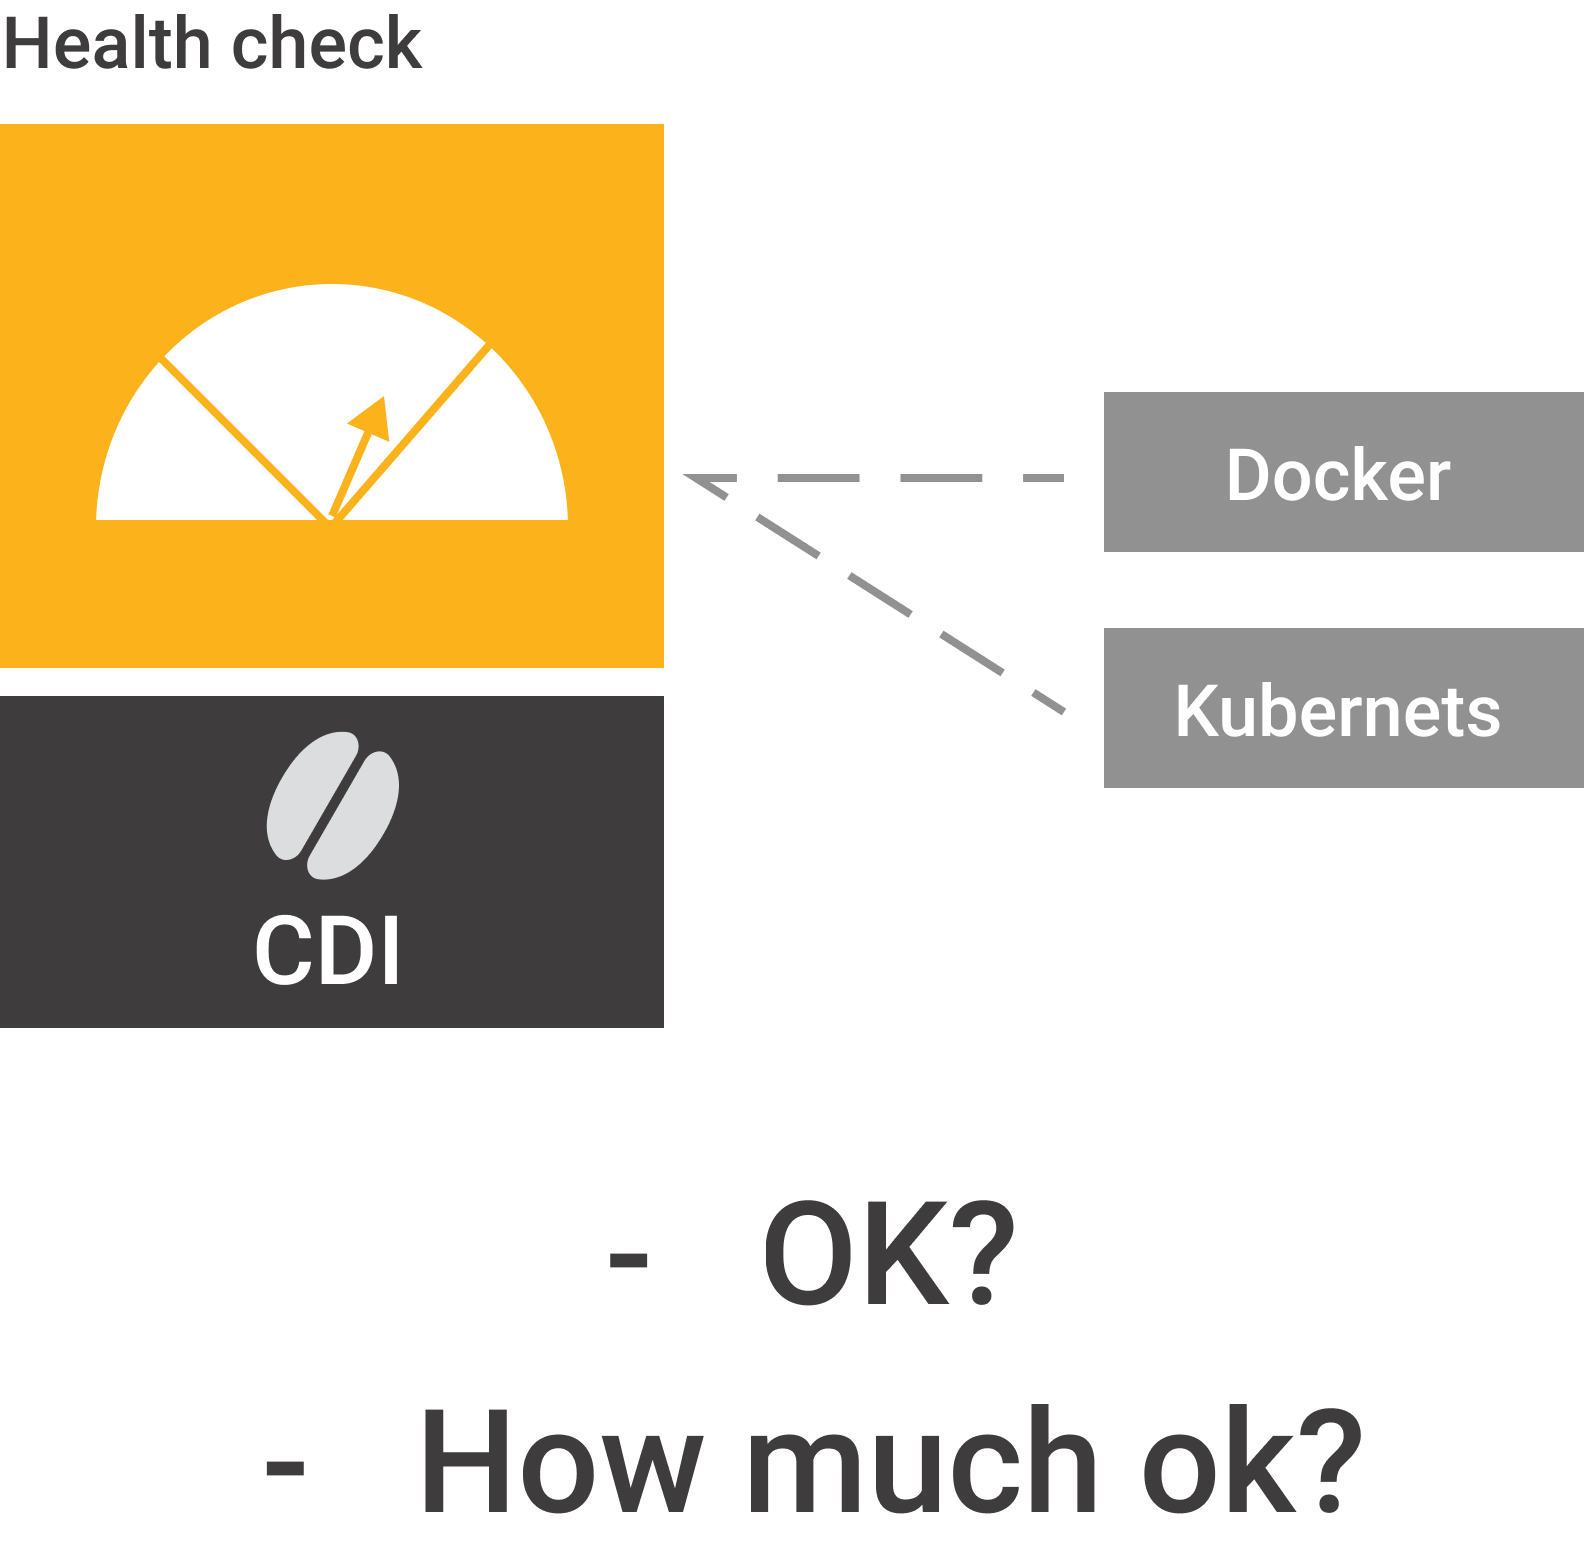
\includegraphics[width=0.75\linewidth]{Images/healthcheck}
\end{figure}
\end{frame}

\begin{frame}[fragile]{Health Check}
¿Estas vivo?
\begin{lstlisting}
@Override
public HealthCheckResponse call() {
	return HealthCheckResponse.named("TaVivoAinda")
		.withData("key1", "val1")
		.withData("key2", "val2")
		.up()
		.build();

}
\end{lstlisting}

\end{frame}


\begin{frame}{JWT}
\begin{figure}
	\centering
	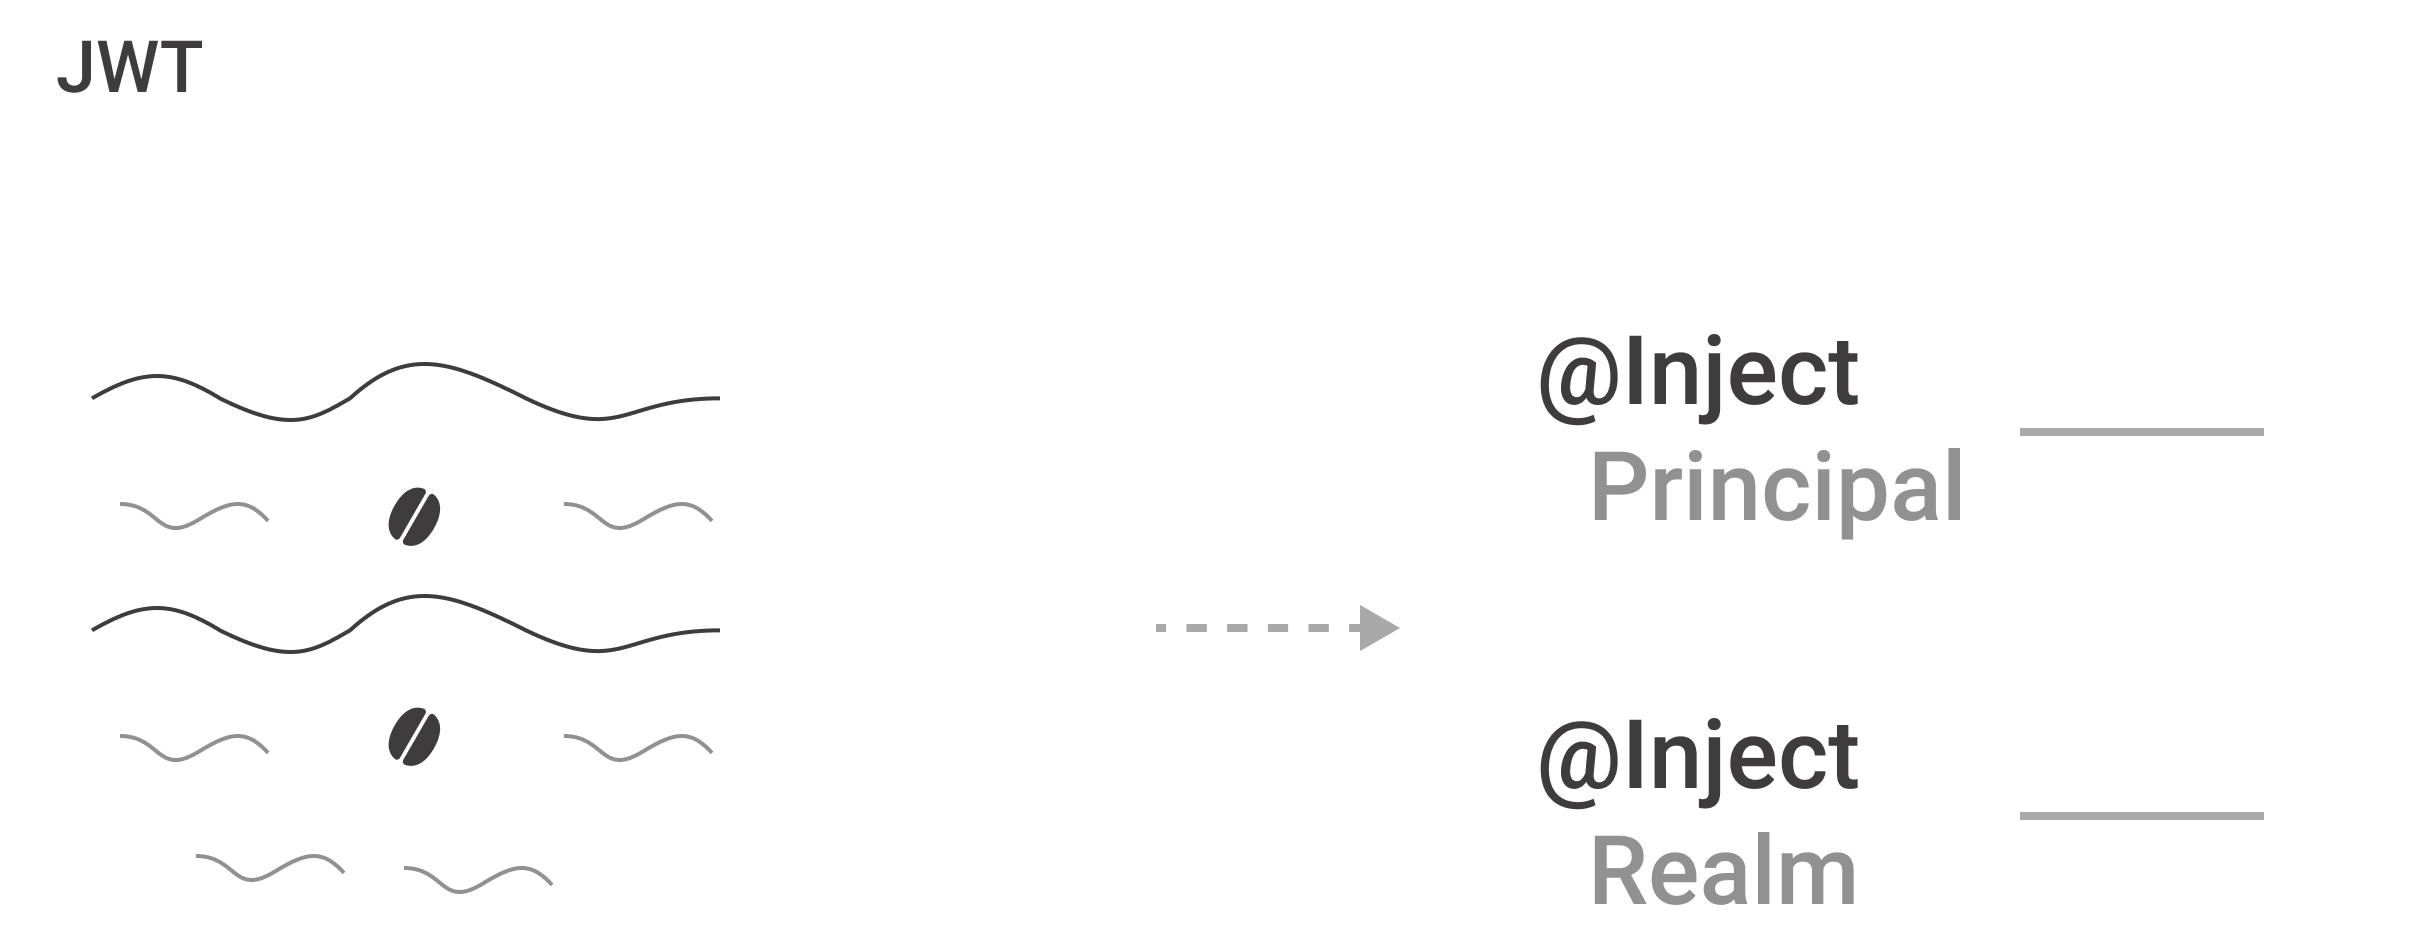
\includegraphics[width=0.9\linewidth]{Images/jwt}
\end{figure}
\end{frame}


\begin{frame}[fragile]{JWT}

\begin{lstlisting}
<@\textcolor{red}{@LoginConfig(authMethod = "MP-JWT")}@>
public class ApplicationConfig extends Application {
}
\end{lstlisting}

\begin{lstlisting}
@Inject
private JsonWebToken jwtPrincipal;

@Inject
<@\textcolor{red}{@Claim("email")}@>
private String email;
\end{lstlisting}
\end{frame}

\begin{frame}{TypeSafe}
\begin{figure}
	\centering
	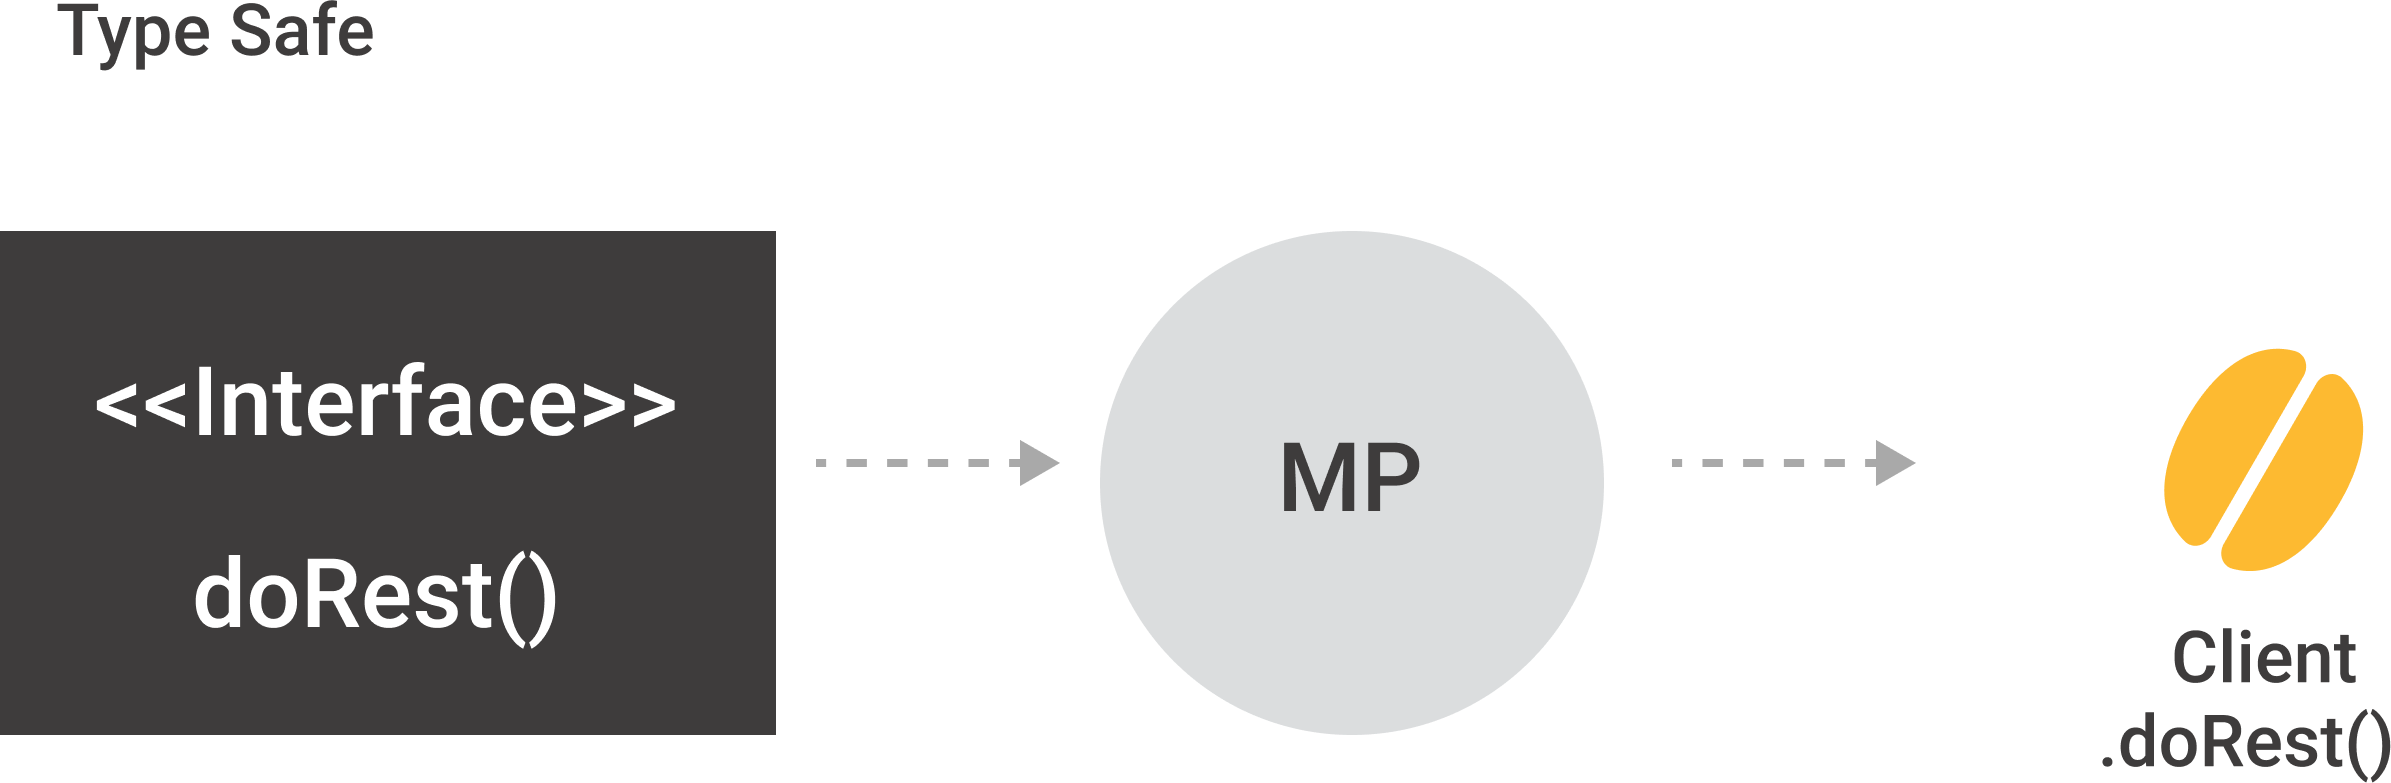
\includegraphics[width=0.75\linewidth]{Images/typesafe}
\end{figure}
\end{frame}

\begin{frame}[fragile]{TypeSafe}


\begin{lstlisting}
@Path("/playlist")
@Consumes("application/json")
public <@\textcolor{red}{interface}@> MusicPlaylistService {

	@GET
	List<String> getPlaylistNames();


	@PUT
	@Path("/{playlistName}")
	long updatePlayList(@PathParam("playlistName")
		String name,
		List<Song> playlist)
		throws UnknownPlaylistException;
}
\end{lstlisting}
\end{frame}


\section{Demo}
\begin{frame}{EE + MicroProfile  - Demo}
\huge Java 11, JAX-RS, CDI, EJB, MicroProfile

\normalsize  \url{https://github.com/tuxtor/payara-demo}\\
\normalsize  \url{https://github.com/tuxtor/omdb-demo}
\end{frame}

\begin{frame}{Payara Micro - Java EE 8}
Stacks tradicionales
\begin{columns}[T] % contents are top vertically aligned
\begin{column}[T]{3cm} % each column can also be its own environment
	\begin{itemize}
		\item EJB
		\item \textbf{JTA}
		\item JAX-RS
		\item CDI
	\end{itemize}
\end{column}
\begin{column}[T]{7cm} % alternative top-align that's better for graphics
	\begin{figure}
		\centering
		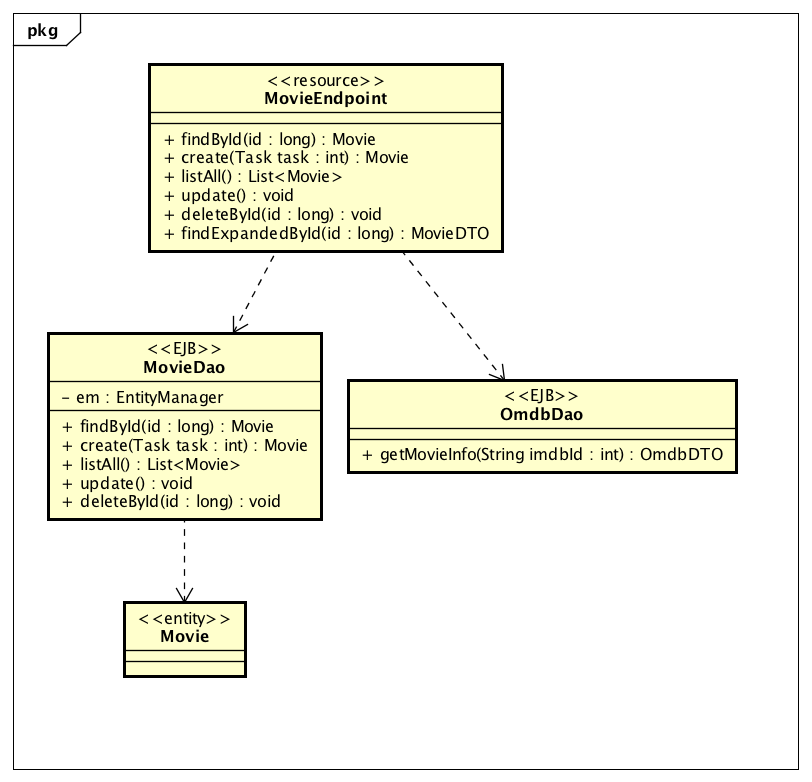
\includegraphics[width=0.9\linewidth]{Images/democlass}
	\end{figure}
\end{column}
\end{columns}
\end{frame}

\begin{frame}{EE + MicroProfile - Demo}
\footnotesize MicroProfile: JAX-RS, CDI, Config, Fault Tolerance, Metrics\\
Payara Micro: EJB, JTA\\
Fatores externos: Location, Deployment, Orchestation, Balancing, Consistency
\begin{figure}
\centering
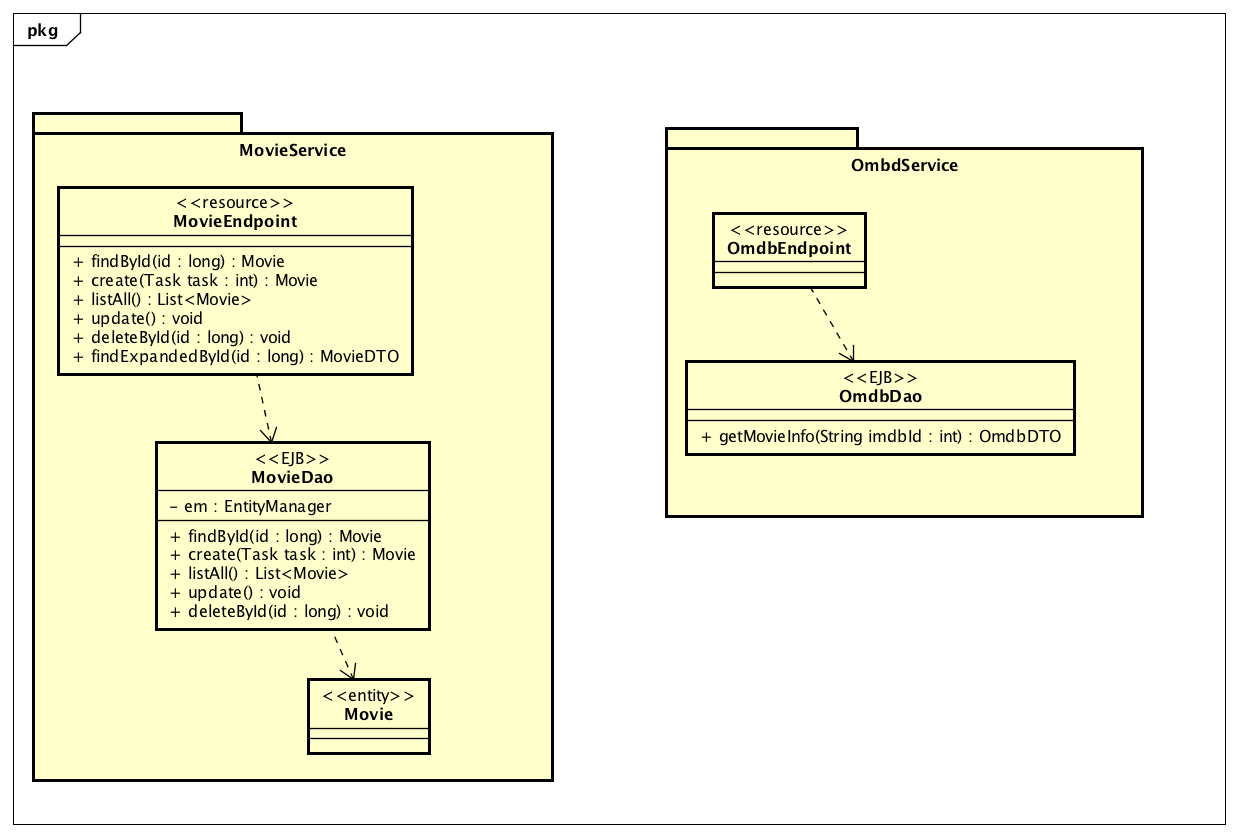
\includegraphics[width=0.65\linewidth]{Images/demomicro}
\end{figure}
\end{frame}

\begin{frame}{12 factores cloud native (Heroku)}

\begin{columns}[T] % contents are top vertically aligned

	\begin{column}[T]{4cm} % alternative top-align that's better for graphics
		\begin{alertblock}{Microprofile}
	\begin{itemize}
		\item Config
		\item Backing service
		\item Disposability
	\end{itemize}
\end{alertblock}
	\end{column}
	\begin{column}[T]{6cm} % each column can also be its own environment
		\begin{block}{Cloud}
	\begin{itemize}
	\item Codebase (Git-Flow)
	\item Dependencies (Maven)
	\item Build, Release, Run
	\item Processes (Pipelines)
	\item Port binding
	\item Concurrency (Docker - k8s)
	\item Dev / Prod parity
	\item Logs
	\item Admin process
\end{itemize}
\end{block}
	\end{column}
\end{columns}

\end{frame}



{
    \usebackgroundtemplate{
\includegraphics[width=\paperwidth]{Images/final}}
    \begin{frame}
    \end{frame}
}


\end{document}
